%% \documentclass[handout,t]{beamer} % HANDOUT
%% \documentclass[handout,notes=show,t]{beamer} % NOTES
\documentclass[t]{beamer} % SLIDES
\usepackage{etex}

\usetheme{DSM}
\usepackage{beamer-tools-dsm}

\input{lib/math}  % basic mathematical notation
\input{lib/text}  % some useful macros for plain text
\input{lib/stat}  % notation for probability theory and statistics
\input{lib/vector}% convenience macros for vectors and matrices

%%%
%%% local configuration adjustments
%%%

%%% You can change pre-defined colours here, override built-in macros from the
%%% style definition and standard library, as well as define macros needed by
%%% all local documents.

%%% e.g. adjust counterpoint (dark green) for data projectors where greens are
%%% far too bright, as well as green component of light colour and pure green
%%% (of course, it's a better solution to adjust the gamma settings of your monitor)
%%
%% \definecolor{counterpoint}{rgb}{.1, .3, 0}
%% \definecolor{light}{rgb}{.45, .3, .55}
%% \definecolor{puregreen}{rgb}{0, .35, 0}

%% ----- extra packages we need to load

\usepackage{tikz}
\usepackage{alltt}              % code examples with nicely formatted comments
\usepackage{hieroglf}           % hieroglyph font for the archeology example
\usepackage{rotating}
\usepackage{multirow}

\usetikzlibrary{arrows.meta}
\usetikzlibrary{shadows}

%% ----- predefined TikZ styles

%% diagram:
%%   box[=colour]   ... shaded text box with drop shadow
%%   arrow[=colour] ... thick arrow between boxes
%%   ghost          ... invisible box (white)
\tikzstyle{diagram box}[secondary]=[
rectangle, rounded corners=1ex, inner sep=5pt, minimum height=4ex, minimum width=4ex,
thick, draw=#1, top color=#1!5!white, bottom color=#1!25!white, drop shadow]

\tikzstyle{diagram ghost}=[
rectangle, rounded corners=1ex, inner sep=5pt, minimum height=4ex, minimum width=4ex,
thick, draw=white, color=white]

\tikzstyle{diagram arrow}[secondary]=[
->, >={Latex[width=4pt, length=4pt]}, ultra thick, color=#1]


%% ----- general copyright message (authors may change between versions of the tutorial)
\newcommand{\dsmcopyright}{%
  Copyright \textcopyright\ 2009--2016 Evert, Lenci, Baroni \& Lapesa | 
  Licensed under CC-by-sa version 3.0}


%% ----- automatically show TOC reminder at beginning of each subsection
\AtBeginSubsection[]
{
  \begin{frame}
    \frametitle{Outline}
    \tableofcontents[current,currentsubsection]
  \end{frame}
}

%% ----- some useful macros for the SIGIL course

%% \begin{Rcode} .. \end{Rcode}
\newenvironment{Rcode}[1][]{%
\setbeamercolor{block title}{fg=counterpoint,bg=counterpoint!15!white}%
\setbeamercolor{block body}{bg=counterpoint!5!white}\small%
\begin{block}{#1}\begin{alltt}\ungap[1]}{%
\ungap[1]\end{alltt}\end{block}}

%% > plot(x,y)      \REM{this produces a scatterplot}
\newcommand{\REM}[2][\small]{\textsf{#1\color{primary}\# #2}}

%% nice colour for R output: \begin{Rout} .. \end{Rout}
\newenvironment{Rout}[1][\footnotesize]{%
  \begin{footnotesize}#1\color{secondary}\bfseries}{%
  \color{black}\mdseries\end{footnotesize}}

%% symbols for centroid vector and singular value matrix 
%% \newcommand{\vmu}[1][]{\boldsymbol{\mu}\ifthenelse{\equal{#1}{}}{}{^{(#1)}}}
\newcommand{\Msigma}{\boldsymbol{\Sigma}}

%% rotated column labels for table (to fit long text into narrow columns
\newcommand{\rotLabel}[2][60]{\begin{rotate}{#1}#2\end{rotate}}

 % local adjustments to configuration and macros

%%%%%%%%%%%%%%%%%%%%%%%%%%%%%%%%%%%%%%%%%%%%%%%%%%%%%%%%%%%%%%%%%%%%%%
%% Titlepage

\title[DSM Tutorial -- Part 1]{Distributional Semantic Models}
\subtitle{Part 1: Introduction}
\author[\textcopyright\ Evert/Baroni/Lenci]{%
  Stefan Evert\inst{1}\\
  {\small with contributions from Marco Baroni\inst{2} and Alessandro Lenci\inst{3}}}
\institute[CC-by-sa]{%
  \inst{1}Friedrich-Alexander-Universität Erlangen-Nürnberg, Germany\\
  \inst{2}University of Trento, Italy\\
  \inst{3}University of Pisa, Italy
}

\date[wordspace.collocations.de]{
  \href{http://wordspace.collocations.de/doku.php/course:start}{\primary{\small http://wordspace.collocations.de/doku.php/course:start}}\\
  \light{\tiny \dsmcopyright}}

\begin{document}

\showLogo
\frame{\titlepage}
\hideLogo

%%%%%%%%%%%%%%%%%%%%%%%%%%%%%%%%%%%%%%%%%%%%%%%%%%%%%%%%%%%%%%%%%%%%%%

\section*{Outline}
\frame{ 
  \frametitle{Outline}
  \tableofcontents
}

%%%%%%%%%%%%%%%%%%%%%%%%%%%%%%%%%%%%%%%%%%%%%%%%%%%%%%%%%%%%%%%%%%%%%%
\section{Introduction}

%%%%%%%%%%%%%%%%%%%%%%%%%%%%%%%%%%%%%%%%%%
\subsection{The distributional hypothesis}

\begin{frame}[c]
  \frametitle{Meaning \& distribution}
  % \framesubtitle{}

  \begin{itemize}
  \item ``Die Bedeutung eines Wortes liegt in seinem Gebrauch.''\\
    \hfill --- Ludwig Wittgenstein
  \item[]
  \item ``You shall know a word by the company it keeps!''\\
    \hfill --- J.~R.\ \citet{Firth:57}
  \item[]
  \item Distributional hypothesis: difference of meaning correlates with difference of distribution \citep[Zellig][]{Harris:54}
  \item[]
  \item ``What people know when they say that they know a word is not how to recite its dictionary definition -- they know how to use it [\ldots] in everyday discourse.'' \citep{Miller:86}
  \end{itemize}
\end{frame}

\begin{frame}
  \frametitle{What is the meaning of ``\textbf{bardiwac}''?}
  % \framesubtitle{}

  \begin{itemize}
  \item<2-> He handed her her glass of \primary{bardiwac}.
  \item<3-> Beef dishes are made to complement the \primary{bardiwacs}.
  \item<4-> Nigel staggered to his feet, face flushed from too much \primary{bardiwac}.
  \item<5-> Malbec, one of the lesser-known \primary{bardiwac} grapes, responds well to Australia's sunshine.
  \item<6-> I dined off bread and cheese and this excellent \primary{bardiwac}.
  \item<7-> The drinks were delicious: blood-red \primary{bardiwac} as well as light, sweet Rhenish.
  \item[\hand]<8-> bardiwac is a heavy red alcoholic beverage made from grapes
  \end{itemize}

  \gap
  \begin{small}
    \visible<8->{\light{The examples above are handpicked, of course.  But in a corpus like the BNC, you will find at least as many informative sentences.}}
  \end{small}
\end{frame}

\begin{frame}[c]
  \frametitle{What is the meaning of ``\textbf{bardiwac}''?}

  \centering
  \only<beamer:1| handout:0>{\includegraphics[width=10cm]{img/SE_bardiwac_conc}}%
  \only<beamer:2| handout:1>{\includegraphics[width=10cm]{img/SE_bardiwac_sketch}}%
\end{frame}

{\newcommand{\hg}[1]{\scriptsize\textpmhg{#1}}
\newcommand<>{\colA}[1]{\purered#2{#1}}
\newcommand<>{\colB}[1]{\puregreen#2{\textbf#2{#1}}}
\begin{frame}<beamer:1-4| handout:1-4>
  \frametitle{A thought experiment: deciphering hieroglyphs}
  % \framesubtitle{}

  \begin{center}
    \setlength{\arrayrulewidth}{1pt}
    \begin{tabular}{@{\rule{0mm}{1.2em} }lr*{6}{|c}|}
      && \hg{get} & \hg{sij} & \hg{ius} & \hg{hir} & \hg{iit} & \hg{kil} \\
      \hline
      \colB<beamer:2| handout:2>{(knife)} & \colB<beamer:2| handout:2>{\hg{naif}} & \colB<beamer:2| handout:2>{51} & \colB<beamer:2| handout:2>{20} & \colB<beamer:2| handout:2>{84} &  \colB<beamer:2| handout:2>{0} &  \colB<beamer:2| handout:2>{3} &  \colB<beamer:2| handout:2>{0} \\
      \hline
      \colB<beamer:4| handout:4>{(cat)}   & \colB<beamer:4| handout:4>{\hg{ket}}  &  \colB<beamer:4| handout:4>{52} & \colB<beamer:4| handout:4>{58} &  \colB<beamer:4| handout:4>{4} &  \colB<beamer:4| handout:4>{4} &  \colB<beamer:4| handout:4>{6} & \colB<beamer:4| handout:4>{26} \\
      \hline
      \h{???} & \h{\hg{dog}} & \colA{115} & \colA{83} & \colA{10} & \colA{42} & \colA{33} & \colA{17} \\
      \hline
      (boat)  & \hg{beut} &  59 & 39 & 23 &  4 &  0 &  0 \\
      \hline
      (cup)   & \hg{kap}  &  98 & 14 &  6 &  2 &  1 &  0 \\
      \hline
      \colB<beamer:3| handout:3>{(pig)}  & \colB<beamer:3| handout:3>{\hg{pigij}} &  \colB<beamer:3| handout:3>{12} & \colB<beamer:3| handout:3>{17} &  \colB<beamer:3| handout:3>{3} &  \colB<beamer:3| handout:3>{2} &  \colB<beamer:3| handout:3>{9} & \colB<beamer:3| handout:3>{27} \\
      \hline
      (banana) & \hg{nana} & 11 &  2 &  2 &  0 & 18 &  0 \\
      \hline
    \end{tabular}
    
    \gap[2]\Large
    \only<beamer:2| handout:2>{%
      sim(\colA{\hg{dog}}, \colB{\hg{naif}}) = 0.770 }%
    \only<beamer:3| handout:3>{%
      sim(\colA{\hg{dog}}, \colB{\hg{pigij}}) = 0.939 }%
    \only<beamer:4| handout:4>{%
      sim(\colA{\hg{dog}}, \colB{\hg{ket}}) = 0.961 }%
  \end{center}

  \addnote{Similarity scores are cosine similarities on sparse log-scaled frequencies ($\log (f+1)$).}%
\end{frame}

\begin{frame}
  \frametitle{English as seen by the computer \ldots}
  % \framesubtitle{}

  \begin{center}
    \ungap[1]
    \setlength{\arrayrulewidth}{1pt}
    \begin{tabular}{@{\rule{0mm}{1.2em} }l@{ }r*{6}{|c}|}
      && get & see & use & hear & eat & kill \\
      && \hg{get} & \hg{sij} & \hg{ius} & \hg{hir} & \hg{iit} & \hg{kil} \\
      \hline
      knife & \hg{naif} &  51 & 20 & 84 &  0 &  3 &  0 \\
      \hline
      cat   & \hg{ket}  &  52 & 58 &  4 &  4 &  6 & 26 \\
      \hline
      \h{dog} & \h{\hg{dog}} & \colA{115} & \colA{83} & \colA{10} & \colA{42} & \colA{33} & \colA{17} \\
      \hline
      boat  & \hg{beut} &  59 & 39 & 23 &  4 &  0 &  0 \\
      \hline
      cup   & \hg{kap}  &  98 & 14 &  6 &  2 &  1 &  0 \\
      \hline
      pig  & \hg{pigij} &  12 & 17 &  3 &  2 &  9 & 27 \\
      \hline
      banana & \hg{nana} & 11 &  2 &  2 &  0 & 18 &  0 \\
      \hline
    \end{tabular}
  \end{center}
  \hfill\light{\footnotesize verb-object counts from British National Corpus}
\end{frame}
}

\begin{frame}
  \frametitle{Geometric interpretation}
  % \framesubtitle{}

  \begin{columns}[T]
    \begin{column}{40mm}
      \begin{itemize}
      \item row vector \primary{$\vx_{\text{dog}}$} describes usage of word \emph{dog} in the corpus
      \item can be seen as coordinates of point in $n$-dimensional Euclidean space
       \end{itemize}
    \end{column}
    \begin{column}{75mm}      
      \gap[2]
      \begin{small}
        \setlength{\arrayrulewidth}{1pt}
        \begin{tabular}{r*{6}{|c}|}
          & get & see & use & hear & eat & kill \\
          \hline
          knife &  51 & 20 & 84 &  0 &  3 &  0 \\
          \hline
          cat  &  52 & 58 &  4 &  4 &  6 & 26 \\
          \hline
          \h{dog} & \primary{115} & \primary{83} & \primary{10} & \primary{42} & \primary{33} & \primary{17} \\
          \hline
          boat &  59 & 39 & 23 &  4 &  0 &  0 \\
          \hline
          cup  &  98 & 14 &  6 &  2 &  1 &  0 \\
          \hline
          pig  &  12 & 17 &  3 &  2 &  9 & 27 \\
          \hline
          banana & 11 &  2 &  2 &  0 & 18 &  0 \\
          \hline
        \end{tabular}
      \end{small}

      \begin{center}
        \h{co-occurrence matrix} $\mathbf{M}$
      \end{center}
    \end{column}
  \end{columns}
\end{frame}

\begin{frame}
  \frametitle{Geometric interpretation}
  % \framesubtitle{}

  \begin{columns}[T]
    \begin{column}{40mm}
      \begin{itemize}
      \item row vector \primary{$\vx_{\text{dog}}$} describes usage of word \emph{dog} in the corpus
      \item can be seen as coordinates of point in $n$-dimensional Euclidean space
      \item illustrated for two dimensions:\\ \emph{get} and \emph{use}
      \item \primary{$\vx_{\text{dog}} = (115,10)$}
      \end{itemize}
    \end{column}
    \begin{column}{75mm}      
      \ungap[1]
      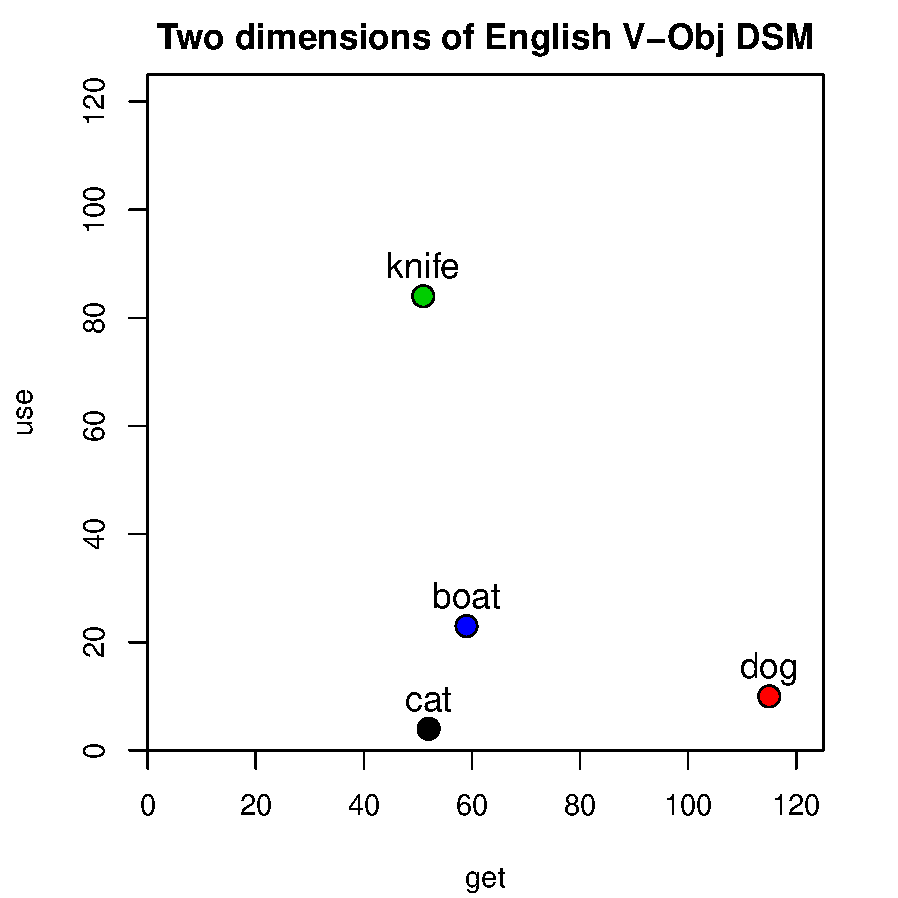
\includegraphics[width=75mm]{img/hieroglyph_2d_1}
    \end{column}
  \end{columns}
\end{frame}

\begin{frame}
  \frametitle{Geometric interpretation}
  % \framesubtitle{}

  \begin{columns}[T]
    \begin{column}{40mm}
      \begin{itemize}
      \item similarity = spatial proximity (Euclidean dist.)
      \item location depends on frequency of noun ($f_{\text{dog}} \approx 2.7\cdot f_{\text{cat}}$)
      \end{itemize}
    \end{column}
    \begin{column}{75mm}      
      \ungap[1]
      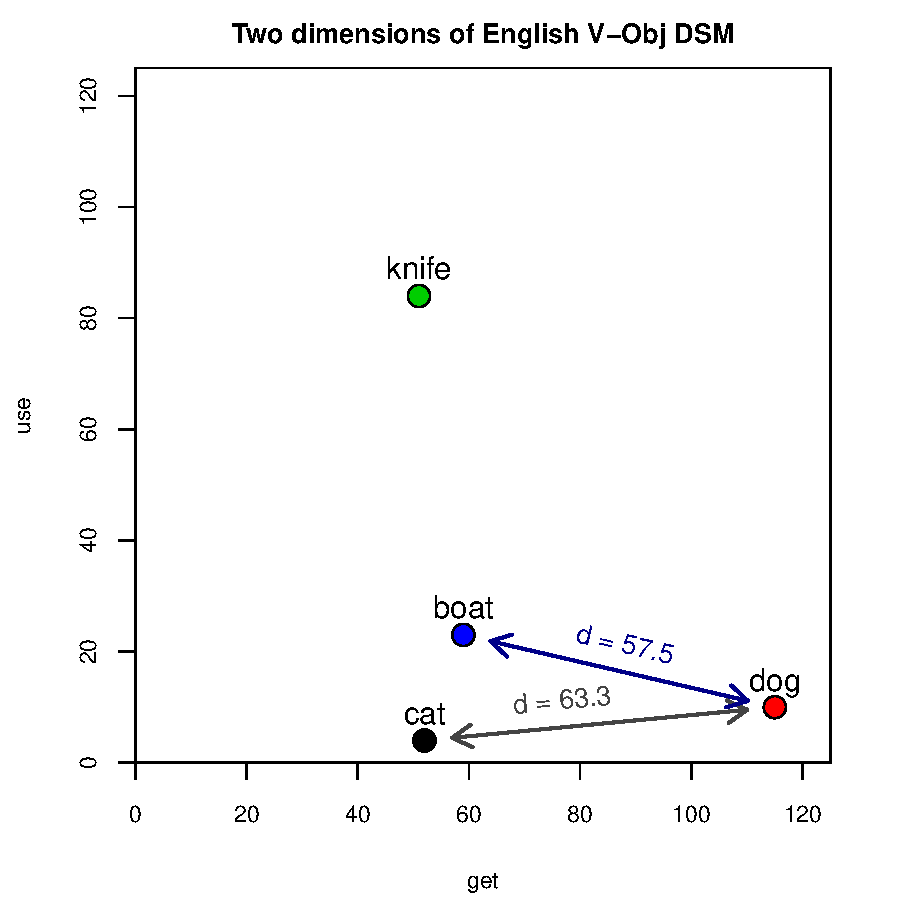
\includegraphics[width=75mm]{img/hieroglyph_2d_2}
    \end{column}
  \end{columns}
\end{frame}

\begin{frame}
  \frametitle{Geometric interpretation}
  % \framesubtitle{}

  \begin{columns}[T]
    \begin{column}{40mm}
      \begin{itemize}
      \item similarity = spatial proximity (Euclidean dist.)
      \item location depends on frequency of noun ($f_{\text{dog}} \approx 2.7\cdot f_{\text{cat}}$)
      \item direction more important than location
      \end{itemize}
    \end{column}
    \begin{column}{75mm}      
      \ungap[1]
      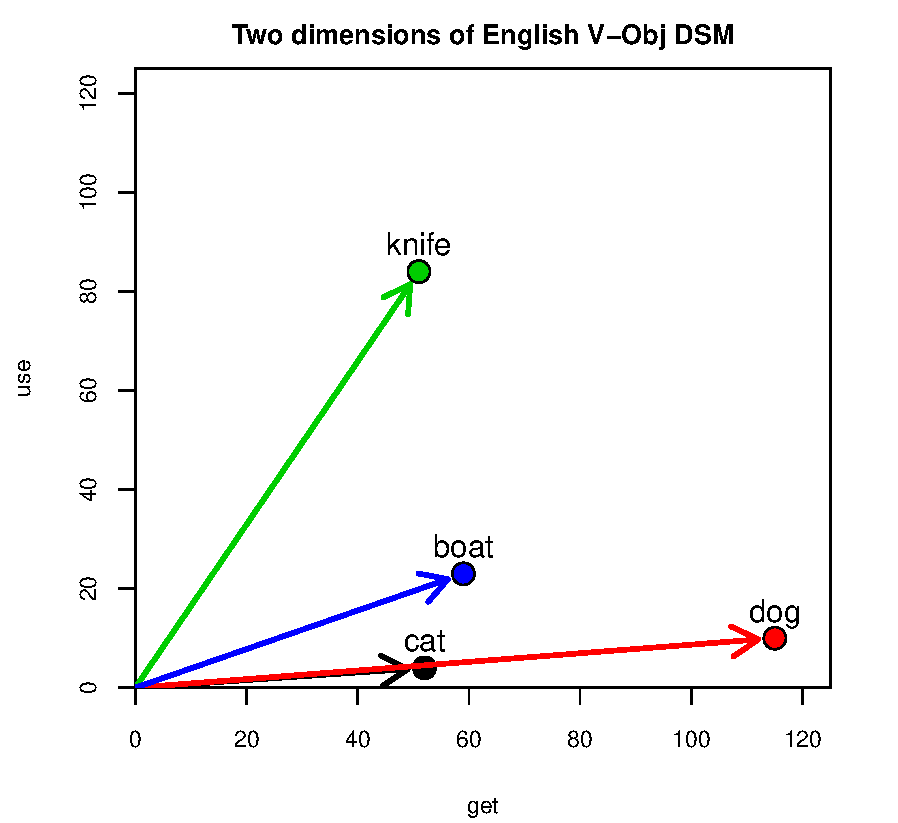
\includegraphics[width=75mm]{img/hieroglyph_2d_3}
    \end{column}
  \end{columns}
\end{frame}

\begin{frame}
  \frametitle{Geometric interpretation}
  % \framesubtitle{}

  \begin{columns}[T]
    \begin{column}{40mm}
      \begin{itemize}
      \item similarity = spatial proximity (Euclidean dist.)
      \item location depends on frequency of noun ($f_{\text{dog}} \approx 2.7\cdot f_{\text{cat}}$)
      \item direction more important than location
      \item<1-> normalise ``length'' $\norm{\vx_{\text{dog}}}$ of vector
      \item<2-> or use angle $\alpha$ as distance measure
      \end{itemize}
    \end{column}
    \begin{column}{75mm}
      \ungap[1]
      \only<beamer:1| handout:0>{%
        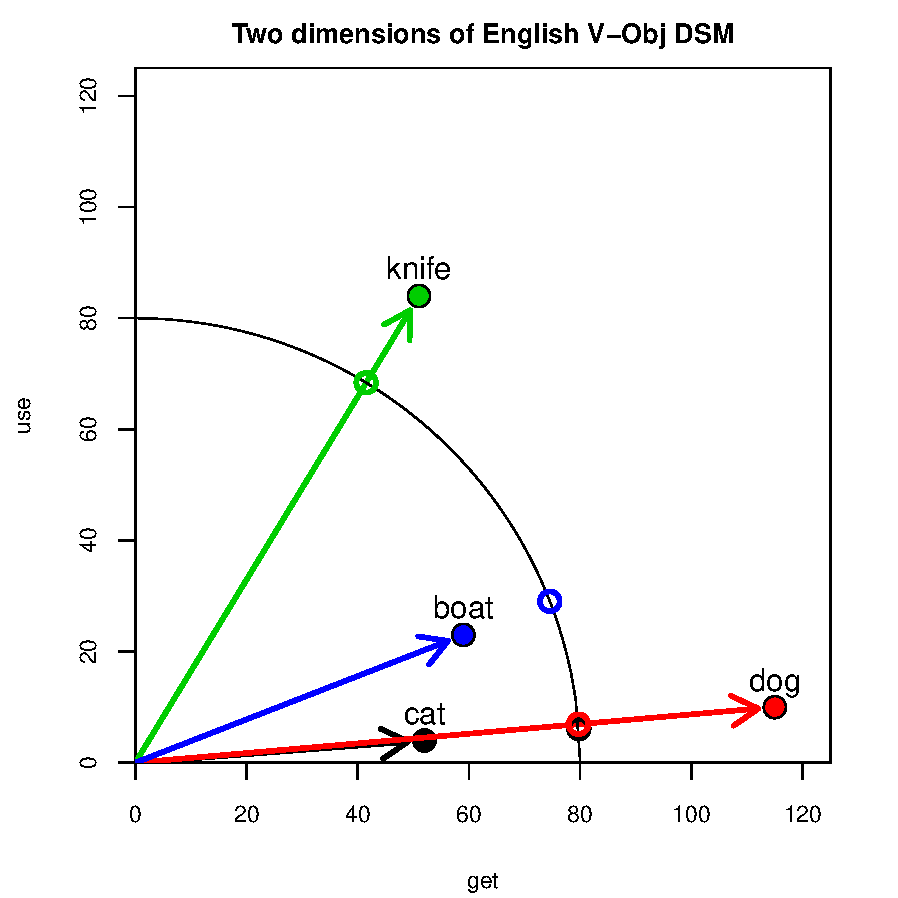
\includegraphics[width=75mm]{img/hieroglyph_2d_4}}%
      \only<beamer:2| handout:1>{%
        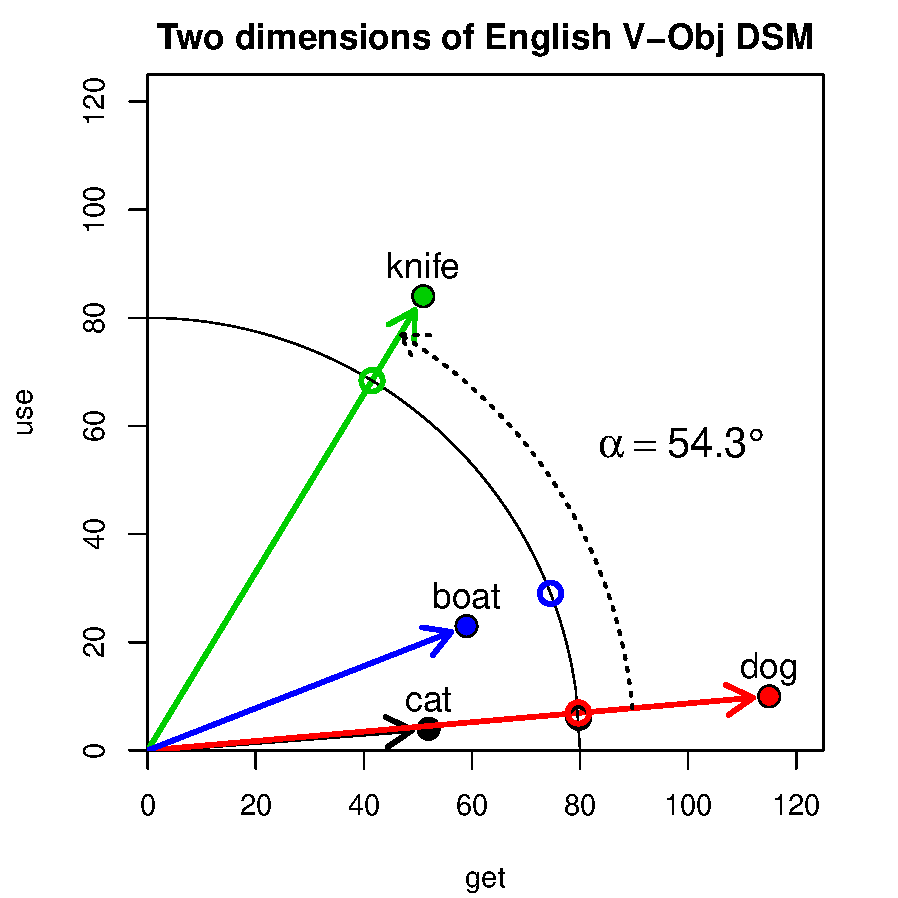
\includegraphics[width=75mm]{img/hieroglyph_2d_5}}%
    \end{column}
  \end{columns}
\end{frame}

\begin{frame}
  \frametitle{Semantic distances}
  % \framesubtitle{}

  \begin{columns}[T]
    \begin{column}{55mm}
      \begin{itemize}
      \item main result of distributional analysis are ``semantic'' distances between words
      \item typical applications
        \begin{itemize}
        \item nearest neighbours
        \item clustering of related words
        \item construct semantic map
        \end{itemize}
      \item other applications require clever use of the distance information
        \begin{itemize}
        \item semantic relations
        \item relational analogies
        \item word sense disambiguation
        \item detection of multiword expressions
        \end{itemize}
      \end{itemize}
    \end{column}
    \begin{column}{55mm}
      \ungap[1]
      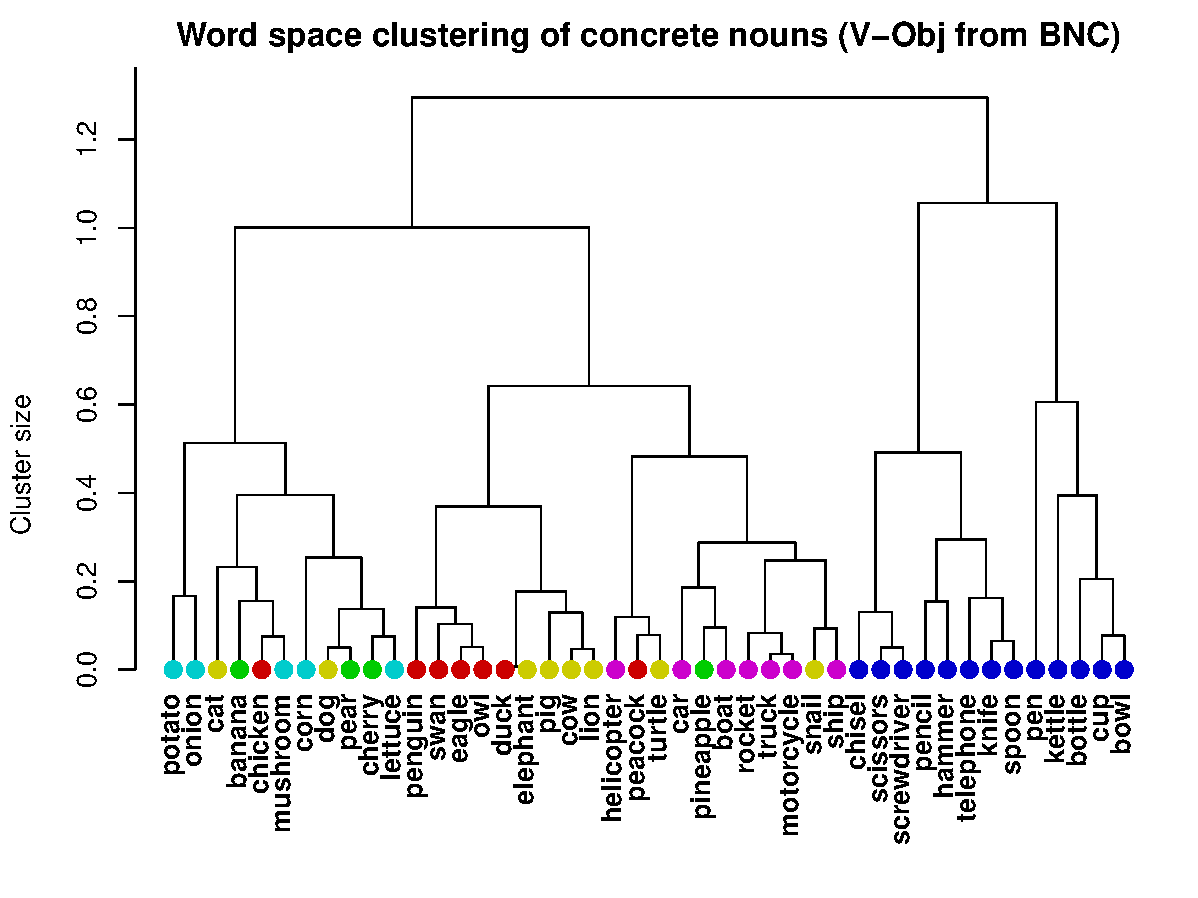
\includegraphics[width=50mm]{img/hieroglyph_clustering}

      \gap[1]
      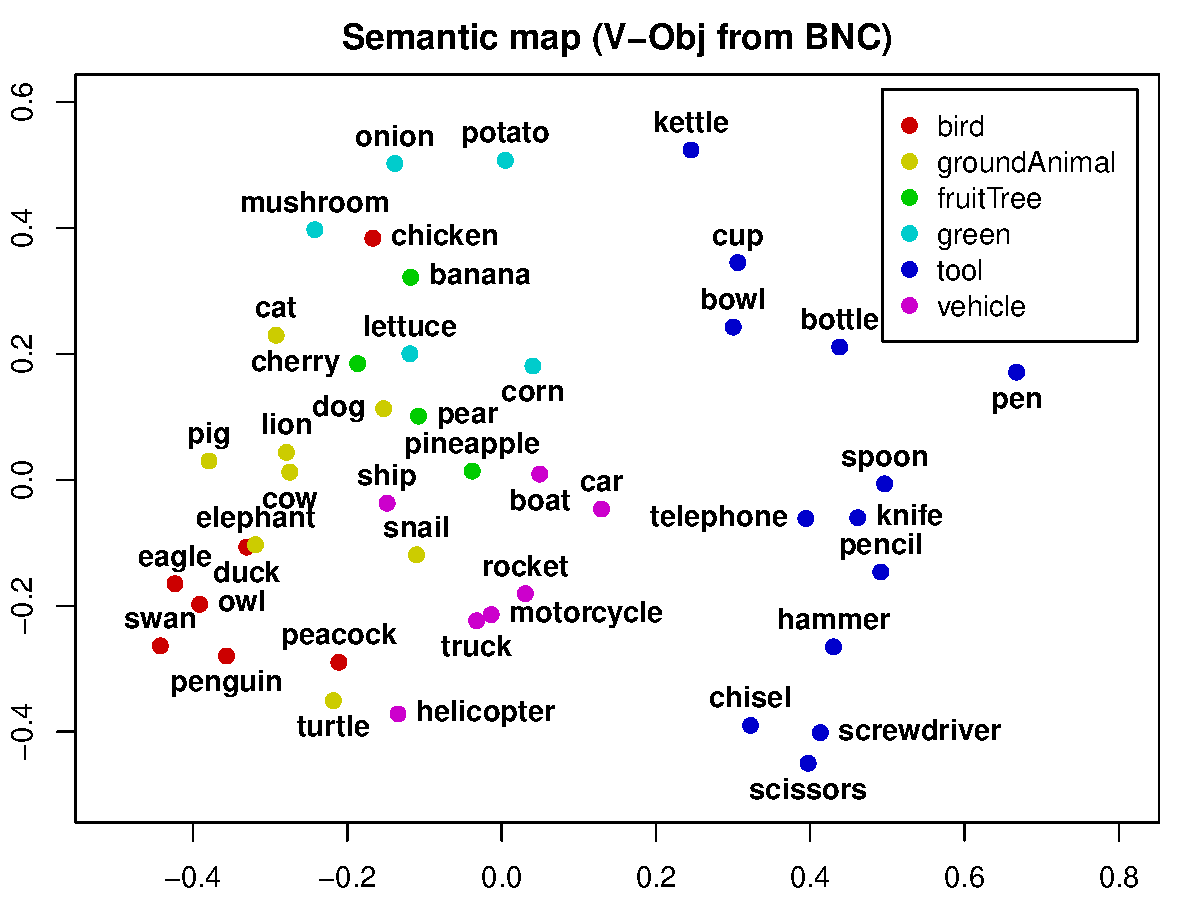
\includegraphics[width=50mm]{img/hieroglyph_semantic_map}
    \end{column}
  \end{columns}
\end{frame}

\begin{frame}
  \frametitle{Some applications in computational linguistics}
  % \framesubtitle{}

  \ungap
  \begin{itemize}
  \item Unsupervised part-of-speech induction \citep{Schuetze:95}
  \item Word sense disambiguation \citep{Schuetze:98}
  \item Query expansion in information retrieval \citep{Grefenstette:94}
  \item Synonym tasks \& other language tests\\\ \citep{Landauer:Dumais:97,Turney:etc:03}
  \item Thesaurus compilation \citep{Lin:98b,Rapp:04a}
  \item Ontology \& wordnet expansion \citep{Pantel:etc:09}
  \item Attachment disambiguation \citep*{Pantel:Lin:00}
  \item Probabilistic language models \citep{Bengio:etc:03b}
  \item Subsymbolic input representation for neural networks
  \item Many other tasks in computational semantics:\\
    entailment detection, noun compound interpretation, identification
    of noncompositional expressions, \ldots
  \end{itemize}
\end{frame}

%%%%%%%%%%%%%%%%%%%%%%%%%%%%%%%%%%%%%%%%%%
\subsection{Three famous DSM examples}

\begin{frame}
  \frametitle{Latent Semantic Analysis \citep{Landauer:Dumais:97}}
  % \framesubtitle{}

  \begin{itemize}
  \item Corpus: 30,473 articles from Grolier's \emph{Academic American Encyclopedia} (4.6 million words in total)
    \begin{itemize}
    \item[\hand] articles were limited to first 2,000 characters
    \end{itemize}
  \item Word-article frequency matrix for 60,768 words
    \begin{itemize}
    \item row vector shows frequency of word in each article
    \end{itemize}
  \item Logarithmic frequencies scaled by word entropy
  \item Reduced to 300 dim.\ by singular value decomposition (SVD)
    \begin{itemize}
    \item borrowed from LSI \citep{Dumais:etc:88}
    \item[\hand] central claim: SVD reveals latent semantic features,\\
      not just a data reduction technique
    \end{itemize}
  \item Evaluated on TOEFL synonym test (80 items)
    \begin{itemize}
    \item LSA model achieved 64.4\% correct answers
    \item also simulation of learning rate based on TOEFL results
    \end{itemize}
  \end{itemize}
\end{frame}

\begin{frame}
  \frametitle{Word Space \citep{Schuetze:92,Schuetze:93,Schuetze:98}}
  % \framesubtitle{}

  \begin{itemize}
  \item Corpus: $\approx 60$ million words of news messages
    \begin{itemize}
    \item from the \emph{New York Times} News Service
    \end{itemize}
  \item Word-word co-occurrence matrix
    \begin{itemize}
    \item 20,000 target words \& 2,000 context words as features
    \item row vector records how often each context word occurs close
      to the target word (co-occurrence)
    \item co-occurrence window: left/right 50 words \citep{Schuetze:98}\\
      or $\approx 1000$ characters \citep{Schuetze:92}
    \end{itemize}
  \item Rows weighted by inverse document frequency (tf.idf)
  \item Context vector = centroid of word vectors (bag-of-words)
    \begin{itemize}
    \item[\hand] goal: determine ``meaning'' of a context
    \end{itemize}
  \item Reduced to 100 SVD dimensions (mainly for efficiency)
  \item Evaluated on unsupervised word sense induction by clustering
    of context vectors (for an ambiguous word)
    \begin{itemize}
    \item induced word senses improve information retrieval performance
    \end{itemize}
  \end{itemize}
\end{frame}

\begin{frame}
  \frametitle{HAL \citep{Lund:Burgess:96}}
  % \framesubtitle{}

  \begin{itemize}
  \item HAL = Hyperspace Analogue to Language
  \item Corpus: 160 million words from newsgroup postings
  \item Word-word co-occurrence matrix
    \begin{itemize}
    \item same 70,000 words used as targets and features
    \item co-occurrence window of 1 -- 10 words
    \end{itemize}
  \item Separate counts for left and right co-occurrence
    \begin{itemize}
    \item i.e.\ the context is \emph{structured}
    \end{itemize}
  \item In later work, co-occurrences are weighted by (inverse) distance \citep{Li:Burgess:Lund:00}
  \item Applications include construction of semantic vocabulary maps
    by multidimensional scaling to 2 dimensions
  \end{itemize}
\end{frame}

\begin{frame}
  \frametitle{Many parameters \ldots}
  % \framesubtitle{}

  \begin{itemize}
  \item Enormous range of DSM parameters and applications
  \item Examples showed three entirely different models, each tuned to
    its particular application
  \item[\So] Need overview of DSM parameters \& understand their effects
  \end{itemize}
\end{frame}

%%%%%%%%%%%%%%%%%%%%%%%%%%%%%%%%%%%%%%%%%%%%%%%%%%%%%%%%%%%%%%%%%%%%%%
\section{Taxonomy of DSM parameters}

%%%%%%%%%%%%%%%%%%%%%%%%%%%%%%%%%%%%%%%%%%
\subsection{Definition \& overview}

\begin{frame}
  \frametitle{General definition of DSMs}
  % \framesubtitle{}

  \ungap
  \begin{block}{}
    A \h{distributional semantic model} (DSM) is a scaled and/or
    transformed co-occurrence matrix $\mathbf{M}$, such that each row $\vx$
    represents the distribution of a target term across contexts.
  \end{block}

  \begin{center}
    \begin{small}
      \setlength{\arrayrulewidth}{1pt}
      \begin{tabular}{r*{6}{|c}|}
        & get & see & use & hear & eat & kill \\
        \hline
        knife &  0.027 & -0.024 &  0.206 & -0.022 & -0.044 & -0.042 \\
        \hline
        cat   &  0.031 &  0.143 & -0.243 & -0.015 & -0.009 &  0.131 \\
        \hline
        \primary{dog}   & \primary{-0.026} &  \primary{0.021} & \primary{-0.212} &  \primary{0.064} &  \primary{0.013} &  \primary{0.014} \\
        \hline
        boat  & -0.022 &  0.009 & -0.044 & -0.040 & -0.074 & -0.042 \\
        \hline
        cup   & -0.014 & -0.173 & -0.249 & -0.099 & -0.119 & -0.042 \\
        \hline
        pig   & -0.069 &  0.094 & -0.158 &  0.000 &  0.094 &  0.265 \\
        \hline
        banana&  0.047 & -0.139 & -0.104 & -0.022 &  0.267 & -0.042 \\
        \hline
      \end{tabular}
    \end{small}
  \end{center}

  \hh{Term} = word, lemma, phrase, morpheme, word pair, \ldots
\end{frame}

\begin{frame}
  \frametitle{General definition of DSMs}
  % \framesubtitle{}

  Mathematical notation:
  \begin{itemize}
  \item $k \times n$ co-occurrence matrix $\mathbf{M}$ (example: $7\times 6$ matrix)
    \begin{itemize}
    \item $k$ rows = target terms
    \item $n$ columns = features or \hh{dimensions}
    \end{itemize}
    \begin{small}
      \gap[.5]
      \[
      \mathbf{M} =
      \begin{bmatrix}
        m_{11} & m_{12} & \cdots & m_{1n} \\
        m_{21} & m_{22} & \cdots & m_{2n} \\
        \vdots & \vdots & & \vdots \\
        m_{k1} & m_{k2} & \cdots & m_{kn}
      \end{bmatrix}
      \]
    \end{small}
  \item distribution vector $\Vector{m}_i$ = $i$-th row of $\mathbf{M}$, e.g.\ $\Vector{m}_3 = \Vector{m}_{\text{dog}}$
  \item components $\Vector{m}_i = (m_{i1}, m_{i2}, \ldots, m_{in})$ = features of $i$-th term:
    \begin{align*}
      \Vector{m}_3 &= (-0.026, 0.021, -0.212, 0.064, 0.013, 0.014) \\
      &= (m_{31}, m_{32}, m_{33}, m_{34}, m_{35}, m_{36})
    \end{align*}
  \end{itemize}

\end{frame}

\begin{frame}
  \frametitle{Overview of DSM parameters}
  % \framesubtitle{}

  \ungap[1]
  \begin{center}
    Term-context \vs\ term-term matrix\\
    \pause $\Downarrow$\\
    Definition of terms \& linguistic pre-processing\\
    \pause $\Downarrow$\\
    Size \& type of context\\
    \pause $\Downarrow$\\
    Geometric \vs\ probabilistic interpretation\\
    \pause $\Downarrow$\\
    Feature scaling\\
    \pause $\Downarrow$\\
    Normalisation of rows and/or columns\\
    \pause $\Downarrow$\\
    Similarity / distance measure\\
    \pause $\Downarrow$\\
    Dimensionality reduction
  \end{center}
\end{frame}

%%%%%%%%%%%%%%%%%%%%%%%%%%%%%%%%%%%%%%%%%%
\subsection{DSM parameters}

\begin{frame}
  \frametitle{Overview of DSM parameters}
  % \framesubtitle{}

  \ungap[1]
  \begin{center}
    \h{Term-context \vs\ term-term matrix}\\
    $\Downarrow$\\
    Definition of terms \& linguistic pre-processing\\
    $\Downarrow$\\
    Size \& type of context\\
    $\Downarrow$\\
    Geometric \vs\ probabilistic interpretation\\
    $\Downarrow$\\
    Feature scaling\\
    $\Downarrow$\\
    Normalisation of rows and/or columns\\
    $\Downarrow$\\
    Similarity / distance measure\\
    $\Downarrow$\\
    Dimensionality reduction
  \end{center}
\end{frame}

\begin{frame}
  \frametitle{Term-context matrix}
  % \framesubtitle{}

  \h{Term-context matrix} records frequency of term in each individual context (e.g.\ sentence, document, Web page, encyclopaedia article)
  
  \gap[3]
  \begin{center}
  \(
  \mathbf{F} = 
  \begin{bmatrix}
    \cdots & \vf_1 & \cdots \\
    \cdots & \vf_2 & \cdots \\
    & \vdots & \\
    & \vdots & \\
    \cdots & \vf_k & \cdots \\
  \end{bmatrix}
  \)
  \hspace{5mm}
  \begin{small}
    \setlength{\arrayrulewidth}{1pt}
    \begin{tabular}[c]{r*{7}{|c}|}
      \multicolumn{1}{c}{}
      & \multicolumn{1}{c}{\rotLabel{Felidae}}
      & \multicolumn{1}{c}{\rotLabel{Pet}}
      & \multicolumn{1}{c}{\rotLabel{Feral}}
      & \multicolumn{1}{c}{\rotLabel{Bloat}}
      & \multicolumn{1}{c}{\rotLabel{Philosophy}}
      & \multicolumn{1}{c}{\rotLabel{Kant}}
      & \multicolumn{1}{c}{\rotLabel{Back pain}} \\
      \cline{2-8}
      cat      &      10 &  10 &     7 &    -- &         -- &   -- &        -- \\
      \cline{2-8}
      dog      &      -- &  10 &     4 &    11 &         -- &   -- &        -- \\
      \cline{2-8}
      animal   &       2 &  15 &    10 &     2 &         -- &   -- &        -- \\
      \cline{2-8}
      time     &       1 &  -- &    -- &    -- &          2 &    1 &        -- \\
      \cline{2-8}
      reason   &      -- &   1 &    -- &    -- &          1 &    4 &         1 \\
      \cline{2-8}
      cause    &      -- &  -- &    -- &     2 &          1 &    2 &         6 \\
      \cline{2-8}
      effect   &      -- &  -- &    -- &     1 &         -- &    1 &        -- \\
      \cline{2-8}
    \end{tabular}
  \end{small}
  \end{center}

\end{frame}

\begin{frame}
  \frametitle{Term-context matrix}
  % \Framesubtitle{}

  Some footnotes:
  \begin{itemize}
  \item Features are usually context \secondary{tokens}, i.e.\ individual instances
  \item Can also be generalised to context \secondary{types}, e.g.
    \begin{itemize}
    \item bag of content words
    \item specific pattern of POS tags 
    \item n-gram of words (or POS tags) around target
    \item subcategorisation pattern of target verb
    \end{itemize}
  \item Term-context matrix is often very \h{sparse}
  \end{itemize}

\end{frame}

\begin{frame}
  \frametitle{Term-term matrix}
  % \framesubtitle{}

  \h{Term-term matrix} records co-occurrence frequencies with feature terms for each target term 

  \gap[2]
  \begin{center}
  \(
  \mathbf{M} = 
  \begin{bmatrix}
    \cdots & \vm_1 & \cdots \\
    \cdots & \vm_2 & \cdots \\
    & \vdots & \\
    & \vdots & \\
    \cdots & \vm_k & \cdots \\
  \end{bmatrix}
  \)
  \hspace{3mm}
  \begin{small}
    \setlength{\arrayrulewidth}{1pt}
    \begin{tabular}[c]{r|c@{$\;$}*{6}{|@{$\;$}c@{$\;$}}|}
      \multicolumn{1}{c}{}
      & \multicolumn{1}{c}{\rotLabel{breed}}
      & \multicolumn{1}{c}{\rotLabel{tail}}
      & \multicolumn{1}{c}{\rotLabel{feed}}
      & \multicolumn{1}{c}{\rotLabel{kill}}
      & \multicolumn{1}{c}{\rotLabel{important}}
      & \multicolumn{1}{c}{\rotLabel{explain}}
      & \multicolumn{1}{c}{\rotLabel{likely}} \\
      \cline{2-8}
      cat     &  83 &  17 &   7 &  37 &  -- &   1 &  -- \\
      \cline{2-8}
      dog     & 561 &  13 &  30 &  60 &   1 &   2 &   4 \\
      \cline{2-8}
      animal  &  42 &  10 & 109 & 134 &  13 &   5 &   5 \\
      \cline{2-8}
      time    &  19 &   9 &  29 & 117 &  81 &  34 & 109 \\
      \cline{2-8}
      reason  &   1 &  -- &   2 &  14 &  68 & 140 &  47 \\
      \cline{2-8}
      cause   &  -- &   1 &  -- &   4 &  55 &  34 &  55 \\
      \cline{2-8}
      effect  &  -- &  -- &   1 &   6 &  60 &  35 &  17 \\
      \cline{2-8}
    \end{tabular}
  \end{small}
  \end{center}

  \begin{itemize}
  \item[\hand] we will usually assume a term-term matrix in this tutorial
  \end{itemize}
\end{frame}

\begin{frame}
  \frametitle{Term-term matrix}
  % \Framesubtitle{}

  Some footnotes:
  \begin{itemize}
  \item Often target terms $\neq$ feature terms
    \begin{itemize}
    \item e.g.\ nouns described by co-occurrences with verbs as features
    \item identical sets of target \& feature terms \so symmetric matrix
    \end{itemize}
  \item Different types of contexts \citep{Evert:08}
    \begin{itemize}
    \item \hh{surface context} (word or character window)
    \item \hh{textual context} (non-overlapping segments)
    \item \hh{syntactic contxt} (specific syntagmatic relation)
    \end{itemize}
  \item Can be seen as smoothing of term-context matrix
    \begin{itemize}
    \item average over similar contexts (with same context terms)
    \item data sparseness reduced, except for small windows
    \item we will take a closer look at the relation between term-context and term-term models later in this tutorial
    \end{itemize}
  \end{itemize}

\end{frame}

\begin{frame}
  \frametitle{Overview of DSM parameters}
  % \framesubtitle{}

  \ungap[1]
  \begin{center}
    Term-context \vs\ term-term matrix\\
    $\Downarrow$\\
    \h{Definition of terms \& linguistic pre-processing}\\
    $\Downarrow$\\
    Size \& type of context\\
    $\Downarrow$\\
    Geometric \vs\ probabilistic interpretation\\
    $\Downarrow$\\
    Feature scaling\\
    $\Downarrow$\\
    Normalisation of rows and/or columns\\
    $\Downarrow$\\
    Similarity / distance measure\\
    $\Downarrow$\\
    Dimensionality reduction
  \end{center}
\end{frame}

\begin{frame}
  \frametitle{Corpus pre-processing}

  \ungap
  \begin{itemize}
  \item Minimally, corpus must be tokenised \so identify terms
  \item Linguistic annotation
    \begin{itemize}
    \item part-of-speech tagging
    \item lemmatisation / stemming
    \item word sense disambiguation (rare)
    \item shallow syntactic patterns
    \item dependency parsing
    \end{itemize}
    \pause
  \item Generalisation of terms
    \begin{itemize}
    \item often lemmatised to reduce data sparseness:\\
      \emph{go, goes, went, gone, going} \so \emph{go}
    \item POS disambiguation (\emph{light}/N \vs\ \emph{light}/A \vs\ \emph{light}/V)
    \item word sense disambiguation (\emph{bank}\tsub{river} \vs\ \emph{bank}\tsub{finance})
    \end{itemize}
  \pause
  \item Trade-off between deeper linguistic analysis and
    \begin{itemize}
    \item need for language-specific resources
    \item possible errors introduced at each stage of the analysis
%%    \item even more parameters to optimise / cognitive plausibility
    \end{itemize}
  \end{itemize}
\end{frame}

\begin{frame}
  \frametitle{Effects of pre-processing}
  \framesubtitle{}

  \centering
  Nearest neighbours of \emph{walk} (BNC)
  \footnotesize
  \begin{columns}[t]
    \column{4cm}
    \begin{block}{word forms}
      \begin{itemize}
      \item stroll
      \item walking
      \item walked
      \item go
      \item path
      \item drive
      \item ride
      \item wander
      \item sprinted
      \item sauntered
      \end{itemize}
    \end{block}
    \column{4cm}
    \begin{block}{lemmatised corpus}
      \begin{itemize}
      \item hurry
      \item stroll
      \item stride
      \item trudge
      \item amble
      \item wander
      \item walk-nn
      \item walking
      \item retrace
      \item scuttle 
      \end{itemize}
    \end{block}
  \end{columns}
\end{frame}

\begin{frame}
  \frametitle{Effects of pre-processing}

  \centering
  Nearest neighbours of \emph{arrivare} (Repubblica)
  \footnotesize
  \begin{columns}[t]
    \column{4cm}
    \begin{block}{word forms}
      \begin{itemize}
      \item  giungere
      \item  \counterpoint{raggiungere}
      \item  \primary{arrivi}
      \item  raggiungimento
      \item  \counterpoint{raggiunto}
      \item  trovare
      \item  \counterpoint{raggiunge}
      \item  \primary{arrivasse}
      \item  \primary{arriver\`a}
      \item  concludere
      \end{itemize}
    \end{block}
    \column{4cm}
    \begin{block}{lemmatised corpus}
      \begin{itemize}
      \item giungere
      \item aspettare
      \item attendere
      \item arrivo-nn
      \item ricevere
      \item accontentare
      \item approdare
      \item pervenire
      \item venire
      \item piombare
      \end{itemize}
    \end{block}
  \end{columns}
  \addnote{Colours seem to indicate inflected forms belonging to the same lemma.}%
\end{frame}

\begin{frame}
  \frametitle{Overview of DSM parameters}
  % \framesubtitle{}

  \ungap[1]
  \begin{center}
    Term-context \vs\ term-term matrix\\
    $\Downarrow$\\
    Definition of terms \& linguistic pre-processing\\
    $\Downarrow$\\
    \h{Size \& type of context}\\
    $\Downarrow$\\
    Geometric \vs\ probabilistic interpretation\\
    $\Downarrow$\\
    Feature scaling\\
    $\Downarrow$\\
    Normalisation of rows and/or columns\\
    $\Downarrow$\\
    Similarity / distance measure\\
    $\Downarrow$\\
    Dimensionality reduction
  \end{center}
\end{frame}

\begin{frame}
  \frametitle{Surface context}
  
  \begin{center}
    Context term occurs \primary{within a window of $k$ words} around target.
  \end{center}

  The {\color{secondary}silhouette of the} \primary{sun}
  {\color{secondary}beyond a wide-open} bay on {\color{secondary}the lake;
    the} \primary{sun} {\color{secondary}still glitters although} evening
  has arrived in Kuhmo. It's midsummer; the living room has its
  instruments and other objects in each of its corners.
  
  \gap
  Parameters:
  \begin{itemize}
  \item window size (in words or characters)
  \item symmetric \vs\ one-sided window
  \item uniform or ``triangular'' (distance-based) weighting
  \item window clamped to sentences or other textual units?
  \end{itemize}
\end{frame}


\begin{frame}
  \frametitle{Effect of different window sizes}
  \framesubtitle{}

  \centering
  Nearest neighbours of \emph{dog} (BNC)
  \footnotesize
  \begin{columns}[t]
    \column{4cm}
    \begin{block}{2-word window}
      \begin{itemize}
      \item cat
      \item horse
      \item fox
      \item pet
      \item rabbit
      \item pig
      \item animal
      \item mongrel
      \item sheep
      \item pigeon
      \end{itemize}
    \end{block}
    \column{4cm}
    \begin{block}{30-word window}
      \begin{itemize}
      \item kennel
      \item puppy
      \item pet
      \item bitch
      \item terrier
      \item rottweiler
      \item canine
      \item cat
      \item to bark
      \item Alsatian
      \end{itemize}
    \end{block}
  \end{columns}
\end{frame}


\begin{frame}
  \frametitle{Textual context}
  
  \begin{center}
    Context term is in the \primary{same linguistic unit} as target.
  \end{center}

  {\color{secondary}The silhouette of the} \primary{sun}
  {\color{secondary}beyond a wide-open bay on the lake; the}
  \primary{sun} {\color{secondary}still glitters although evening has
    arrived in Kuhmo.} It's midsummer; the living room has its
  instruments and other objects in each of its corners.
  
  \gap
  Parameters:
  \begin{itemize}
  \item type of linguistic unit
    \begin{itemize}
    \item sentence
    \item paragraph
    \item turn in a conversation
    \item Web page
    \end{itemize}
  \end{itemize}
\end{frame}

\begin{frame}
  \frametitle{Syntactic context}
  
  \ungap
  \begin{center}
    Context term is linked to target by a \primary{syntactic dependency}\\
    (e.g. subject, modifier, \ldots).
  \end{center}

  The {\color{secondary}silhouette} of the \primary{sun} beyond a
  wide-open {\color{secondary}bay} on the lake; the \primary{sun}
  still {\color{secondary}glitters} although evening has arrived in
  Kuhmo. It's midsummer; the living room has its instruments and other
  objects in each of its corners.
  
  \gap
  Parameters:
  \begin{itemize}
  \item types of syntactic dependency \citep{Pado:Lapata:07}
  \item direct \vs\ indirect dependency paths
    \begin{itemize}
    \item direct dependencies
    \item direct + indirect dependencies
    \end{itemize}
  \item homogeneous data (e.g.\ only verb-object) \vs\\
    heterogeneous data (e.g.\ all children and parents of the verb)
  \item maximal length of dependency path
  \end{itemize}
\end{frame}


\begin{frame}
  \frametitle{``Knowledge pattern'' context}
  
  \begin{center}
    Context term is linked to target by a \primary{lexico-syntactic pattern}\\
    (text mining, cf.\ Hearst 1992, Pantel \& Pennacchiotti 2008, etc.).
  \end{center}  

  In Provence, Van Gogh painted with bright \primary{colors}
  {\color{counterpoint}such as} {\color{secondary}red} {\color{counterpoint}and}
  {\color{secondary}yellow}.  These \primary{colors}
  {\color{counterpoint}produce} incredible {\color{secondary}effects} on
  anybody looking at his paintings.
  
  \gap
  Parameters:
  \begin{itemize}
  \item inventory of lexical patterns
    \begin{itemize}
    \item lots of research to identify semantically interesting patterns (cf. Almuhareb \& Poesio 2004,
      Veale \& Hao 2008, etc.)
    \end{itemize}
  \item fixed \vs\ flexible patterns
    \begin{itemize}
    \item patterns are mined from large corpora and automatically generalised (optional elements, POS tags or semantic classes)
    \end{itemize}
  \end{itemize}
\end{frame}

\begin{frame}[c]
  \frametitle{Structured vs.\ unstructured context}
  % \framesubtitle{}

  \begin{itemize}
  \item In \h{unstructered} models, context specification acts as a \hh{filter}
    \begin{itemize}
    \item determines whether context tokens counts as co-occurrence
    \item e.g.\ linked by specific syntactic relation such as verb-object
    \item[]
    \end{itemize}
    \pause
  \item In \h{structured} models, context words are \hh{subtyped}
    \begin{itemize}
    \item depending on their position in the context
    \item e.g.\ left \vs\ right context, type of syntactic relation, etc.
    \end{itemize}
  \end{itemize}
\end{frame}

\begin{frame}
  \frametitle{Structured \vs\ unstructured surface context}

  A dog bites a man. The man's dog bites a dog.  A dog bites a man.
  
 \begin{center}
    \begin{tabular}{r|c}
      \h{unstructured} &  bite \\
      dog & 4 \\
      man & 3 
    \end{tabular}
  \end{center}

  \gap[2]\pause
  A dog bites a man. The man's dog bites a dog.  A dog bites a man.
  
  \begin{center}
    \begin{tabular}{r|c|c}
      \h{structured} &  bite-l & bite-r \\
      dog & 3 & 1 \\
      man & 1  & 2
    \end{tabular}
  \end{center}
\end{frame}


\begin{frame}
  \frametitle{Structured \vs\ unstructured dependency context}

  A dog bites a man. The man's dog bites a dog.  A dog bites a man.
  
  \begin{center}
    \begin{tabular}{r|c}
      \h{unstructured} &  bite \\
      dog & 4 \\
      man & 2 
    \end{tabular}
  \end{center}

  \gap[2]\pause
  A dog bites a man. The man's dog bites a dog.  A dog bites a man.
  
   \begin{center}
     \begin{tabular}{r|c|c}
       \h{structured} &  bite-subj & bite-obj \\
       dog & 3 & 1 \\
       man & 0  & 2
     \end{tabular}
   \end{center}
\end{frame}


\begin{frame}
  \frametitle{Comparison}

  \begin{itemize}
  \item Unstructured context
    \begin{itemize}
    \item data less sparse (e.g.\ \emph{man kills} and \emph{kills man} both
      map to the \emph{kill} dimension of the vector $\vx_{\text{man}}$)
    \item[]
    \end{itemize}
  \item Structured context
    \begin{itemize}
    \item more sensitive to semantic distinctions\\
      (\emph{kill-subj} and \emph{kill-obj} are rather different
      things!)
    \item dependency relations provide a form of syntactic ``typing''
      of the DSM dimensions (the ``subject'' dimensions, the
      ``recipient'' dimensions, etc.)
     \item important to account for word-order and compositionality 
    \end{itemize}
  \end{itemize}
\end{frame}

\begin{frame}
  \frametitle{Overview of DSM parameters}
  % \framesubtitle{}

  \ungap[1]
  \begin{center}
    Term-context \vs\ term-term matrix\\
    $\Downarrow$\\
    Definition of terms \& linguistic pre-processing\\
    $\Downarrow$\\
    Size \& type of context\\
    $\Downarrow$\\
    \h{Geometric \vs\ probabilistic interpretation}\\
    $\Downarrow$\\
    Feature scaling\\
    $\Downarrow$\\
    Normalisation of rows and/or columns\\
    $\Downarrow$\\
    Similarity / distance measure\\
    $\Downarrow$\\
    Dimensionality reduction
  \end{center}
\end{frame}

\begin{frame}
  \frametitle{Geometric vs.\ probabilistic interpretation}
  % \framesubtitle{}

  \begin{itemize}
  \item Geometric interpretation
    \begin{itemize}
    \item row vectors as points or arrows in $n$-dim.\ space
    \item very intuitive, good for visualisation
    \item use techniques from geometry and linear algebra
    \item[]
    \end{itemize}
    \pause
  \item Probabilistic interpretation
    \begin{itemize}
    \item co-occurrence matrix as observed sample statistic
    \item ``explained'' by generative probabilistic model
    \item recent work focuses on hierarchical Bayesian models
    \item probabilistic LSA \citep{Hoffmann:99}, Latent Semantic
      Clustering \citep{Rooth:etc:99}, Latent Dirichlet Allocation
      \citep{Blei:Ng:Jordan:03}, etc.
    \item explicitly accounts for random variation of frequency counts
    \item intuitive and plausible as topic model
    \item[]
    \end{itemize}
    \pause
  \item[\hand] focus on geometric interpretation in this tutorial
  \end{itemize}
\end{frame}

\begin{frame}
  \frametitle{Overview of DSM parameters}
  % \framesubtitle{}

  \ungap[1]
  \begin{center}
    Term-context \vs\ term-term matrix\\
    $\Downarrow$\\
    Definition of terms \& linguistic pre-processing\\
    $\Downarrow$\\
    Size \& type of context\\
    $\Downarrow$\\
    Geometric \vs\ probabilistic interpretation\\
    $\Downarrow$\\
    \h{Feature scaling}\\
    $\Downarrow$\\
    Normalisation of rows and/or columns\\
    $\Downarrow$\\
    Similarity / distance measure\\
    $\Downarrow$\\
    Dimensionality reduction
  \end{center}
\end{frame}

\begin{frame}
  \frametitle{Feature scaling}

  Feature scaling is used to ``discount'' less important features:
  \begin{itemize}
  \item<1-> Logarithmic scaling: $x' = \log (x+1)$\\
    (cf.\ Weber-Fechner law for human perception)
  \item<2-> Relevance weighting, e.g.\ \secondary{tf.idf} (information retrieval)
  \item<3-> Statistical \h{association measures} \citep{Evert:04phd,Evert:08}
    take frequency of target word and context feature into account
    \begin{itemize}
    \item the less frequent the target word and (more importantly) the
      context feature are, the higher the weight given to their
      observed co-occurrence count should be (because their expected
      chance co-occurrence frequency is low)
    \item different measures -- e.g., mutual information,
      log-likelihood ratio -- differ in how they balance observed and
      expected co-occurrence frequencies
    \end{itemize}
  \end{itemize}
\end{frame}

\begin{frame}
  \frametitle{Association measures: Mutual Information (MI)}

  \begin{center}
    \begin{tabular}{llrrr}
      word\tsub1 & word\tsub2 & $f_{\text{obs}}$ & $f_1$ & $f_2$ \\
      \hline
      \emph{dog} & \emph{small} & 855 &33,338 & 490,580\\ 
      \emph{dog} & \emph{domesticated} & 29 &33,338& 918\\
    \end{tabular}
  \end{center}

  \pause
  Expected co-occurrence frequency:
  \[
  f_{\text{exp}} = \frac{f_1 \cdot f_2}{N}
  \]
  
  \pause
  Mutual Information compares observed \vs\ expected frequency:
  \[
  \text{MI}(w_{1},w_{2}) =
  \log_{2} \frac{f_{\text{obs}}}{f_{\text{exp}}} =
  \log_2 \frac{N\cdot f_{\text{obs}}}{f_1\cdot f_2}
  \]
  
  \pause
  Disadvantage: MI overrates combinations of rare terms.
\end{frame}



\begin{frame}
  \frametitle{Other association measures}

  \ungap[2]
  \begin{center}
    \begin{tabular}{llrrr>{\color{primary}}r>{\color{secondary}}r}
      word\tsub1 & word\tsub2 & $f_{\text{obs}}$ & $f_{\text{exp}}$ & MI & \visible<2->{local-MI} & \visible<3->{t-score} \\
      \hline
      \emph{dog} & \emph{small}        & 855 &   134.34 &  2.67 & \visible<2->{2282.88} & \visible<3->{24.64}\\ 
      \emph{dog} & \emph{domesticated} &  29 &     0.25 &  6.85 & \visible<2->{ 198.76} & \visible<3->{ 5.34}\\
      \emph{dog} & \emph{sgjkj}        &   1 &  0.00027 & 11.85 & \visible<2->{  11.85} & \visible<3->{ 1.00}\\ 
    \end{tabular}
  \end{center}

  \onslide<2->\gap
  The \primary{log-likelihood ratio} \citep{Dunning:93} has more complex form, but
  its ``core'' is known as local MI \citep{Evert:04phd}.

  \[
  \text{local-MI}(w_1, w_2) = f_{\text{obs}} \cdot \text{MI}(w_1, w_2)
  \]
 
  \onslide<3->
  The \secondary{t-score} measure \citep{Church:Hanks:90} is popular in lexicography:
  \[
  \text{t-score}(w_1, w_2) = \frac{f_{\text{obs}} - f_{\text{exp}}}{\sqrt{f_{\text{obs}}}}
  \]

  Details \& many more measures: \secondary{\url{http://www.collocations.de/}}
\end{frame}

\begin{frame}
  \frametitle{Overview of DSM parameters}
  % \framesubtitle{}

  \ungap[1]
  \begin{center}
    Term-context \vs\ term-term matrix\\
    $\Downarrow$\\
    Definition of terms \& linguistic pre-processing\\
    $\Downarrow$\\
    Size \& type of context\\
    $\Downarrow$\\
    Geometric \vs\ probabilistic interpretation\\
    $\Downarrow$\\
    Feature scaling\\
    $\Downarrow$\\
    \h{Normalisation of rows and/or columns}\\
    $\Downarrow$\\
    Similarity / distance measure\\
    $\Downarrow$\\
    Dimensionality reduction
  \end{center}
\end{frame}

\begin{frame}[c]
  \frametitle{Normalisation of row vectors}
  % \framesubtitle{}
  
  \begin{columns}[c]
    \begin{column}{5cm}
      \begin{itemize}
      \item geometric distances only make sense if vectors are normalised to unit length
      \item divide vector by its length: \[ \vx / \norm{\vx} \]
      \item normalisation depends on distance measure!
      \item special case: scale to relative frequencies with
        $\norm[1]{\vx} = \abs{x_1} + \dots + \abs{x_n}$\\
        \so probabilistic interpretation
      \end{itemize}
    \end{column}
    \begin{column}{6cm}
      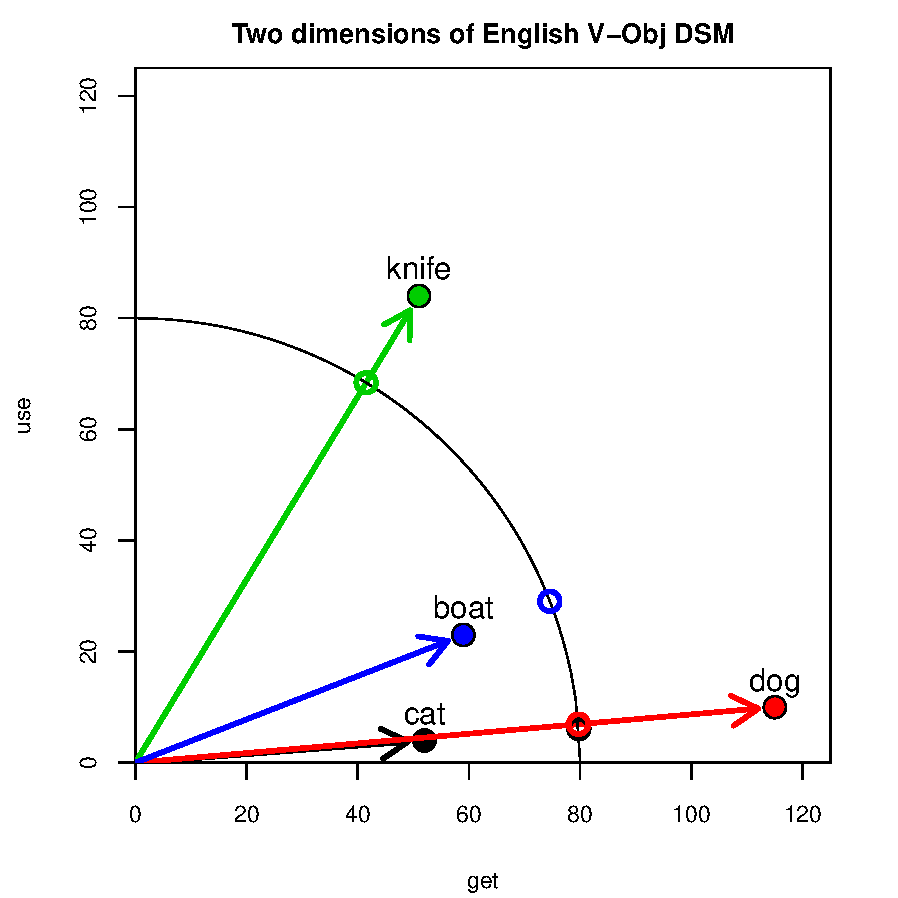
\includegraphics[width=6cm]{img/hieroglyph_2d_4}
    \end{column}
  \end{columns}
\end{frame}

\begin{frame}
  \frametitle{Scaling of column vectors}
  % \framesubtitle{}

  \begin{itemize}
  \item In statistical analysis and machine learning, features are
    usually \primary{centred} and \primary{scaled} so that
    \begin{align*}
      \text{mean} & \quad \mu = 0 \\
      \text{variance} & \quad \sigma^2 = 1
    \end{align*}
  \item In DSM research, this step is less common for columns of $\mathbf{M}$
    \begin{itemize}
    \item centring is a prerequisite for certain dimensionality
      reduction and data analysis techniques (esp.\ PCA)
    \item scaling may give too much weight to rare features
    \end{itemize}
    \pause
  \item $\mathbf{M}$ cannot be row-normalised and column-scaled at the
    same time (result depends on ordering of the two steps)
  \end{itemize}
\end{frame}

\begin{frame}
  \frametitle{Overview of DSM parameters}
  % \framesubtitle{}

  \ungap[1]
  \begin{center}
    Term-context \vs\ term-term matrix\\
    $\Downarrow$\\
    Definition of terms \& linguistic pre-processing\\
    $\Downarrow$\\
    Size \& type of context\\
    $\Downarrow$\\
    Geometric \vs\ probabilistic interpretation\\
    $\Downarrow$\\
    Feature scaling\\
    $\Downarrow$\\
    Normalisation of rows and/or columns\\
    $\Downarrow$\\
    \h{Similarity / distance measure}\\
    $\Downarrow$\\
    Dimensionality reduction
  \end{center}
\end{frame}

\begin{frame}
  \frametitle{Geometric distance}
  %% \framesubtitle{}

  \begin{columns}[T]
    \begin{column}{60mm}
      \begin{itemize}
      \item \h{Distance} between vectors $\vu, \vv \in \setR^n$ \so
        (dis)\h{similarity}
        \begin{itemize}
        \item $\vu = (u_1, \ldots, u_n)$
        \item $\vv = (v_1, \ldots, v_n)$
        \end{itemize}
      \item<2-> \h{Euclidean} distance $\dist[2]{\vu}{\vv}$
      \item<3-> ``City block'' \h{Manhattan} distance $\dist[1]{\vu}{\vv}$
      \item<4-> Both are special cases of the \h{Minkowski} $p$-distance
        $\dist[p]{\vu}{\vv}$ (for $p\in [1, \infty]$)
      \end{itemize}
    \end{column}
    \begin{column}{45mm}
      \includegraphics[width=45mm]{img/2_distance_examples}
    \end{column}
  \end{columns}
  \gap[.5]
  \only<beamer:2| handout:0>{%
    \[ \dist[2]{\vu}{\vv} \coloneq \sqrt{(u_1 - v_1)^2 + \dots + (u_n - v_n)^2} \] }
  \only<beamer:3| handout:0>{%
    \[ \dist[1]{\vu}{\vv} \coloneq \abs{u_1 - v_1} + \dots + \abs{u_n - v_n} \] }
  \only<beamer:4-| handout:1>{%
    \[ \dist[p]{\vu}{\vv} \coloneq \bigl(
    \abs{u_1 - v_1}^p + \dots + \abs{u_n - v_n}^p
    \bigr)^{1/p} \] }
  \only<beamer:5-| handout:1>{%
    \[ \dist[\infty]{\vu}{\vv} = \max \bigset{\abs{u_1 - v_1}, \ldots, \abs{u_n - v_n}} \] }
\end{frame}


\begin{frame}
  \frametitle{Other distance measures}
  % \framesubtitle{}
  
  \begin{itemize}
  \item Information theory: \h{Kullback-Leibler} (KL) \h{divergence} for probability vectors (non-negative, $\norm[1]{\vx} = 1$)
    \[
    \KL{\vu}{\vv} = \sum_{i=1}^n u_i \cdot \log_2 \frac{u_i}{v_i}
    \]
    \pause
  \item Properties of KL divergence
    \begin{itemize}
    \item most appropriate in a probabilistic interpretation of $\mathbf{M}$
    \item zeroes in $\vv$ without corresponding zeroes in $\vu$ are problematic
    \item not symmetric, unlike geometric distance measures
    \item alternatives: skew divergence, Jensen-Shannon divergence
    \item[]
    \end{itemize}
    \pause
  \item A symmetric distance measure \citep{Endres:Schindelin:03}
    \[
    D_{\vu\vv} = \KL{\vu}{\vz} + \KL{\vv}{\vz} \quad \text{with} \quad \vz = \frac{\vu + \vv}{2}
    \]
  \end{itemize}
\end{frame}

\begin{frame}
  \frametitle{Similarity measures}
  % \framesubtitle{}
  
  \begin{columns}[c]
    \begin{column}{5cm}
      \begin{itemize}
        \item angle $\alpha$ between two vectors $\vu,\vv$ is given by
          \begin{align*}
            \cos \alpha &= 
            \frac{\sum_{i=1}^n u_i\cdot v_i}{
              \sqrt{\sum_i u_i^2}\cdot \sqrt{\sum_i v_i^2}}
            \\
            &= \frac{\sprod{\vu}{\vv}}{\norm[2]{\vu}\cdot \norm[2]{\vv}}
        \end{align*}
      \item<2-> \h{cosine} measure of similarity: $\cos \alpha$
        \begin{itemize}
        \item $\cos \alpha = 1$ \so collinear
        \item $\cos \alpha = 0$ \so orthogonal
        \end{itemize}
      \end{itemize}
    \end{column}
    \begin{column}{6cm}
      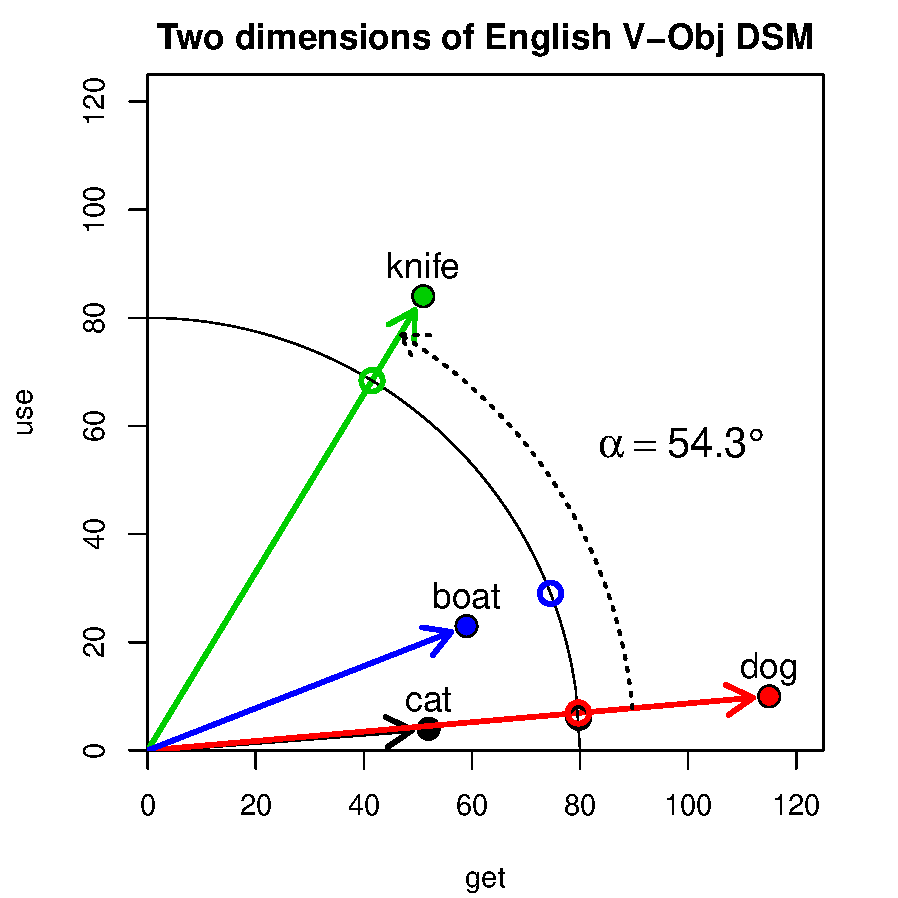
\includegraphics[width=6cm]{img/hieroglyph_2d_5}
    \end{column}
  \end{columns}
\end{frame}

\begin{frame}
  \frametitle{Overview of DSM parameters}
  % \framesubtitle{}

  \ungap[1]
  \begin{center}
    Term-context \vs\ term-term matrix\\
    $\Downarrow$\\
    Definition of terms \& linguistic pre-processing\\
    $\Downarrow$\\
    Size \& type of context\\
    $\Downarrow$\\
    Geometric \vs\ probabilistic interpretation\\
    $\Downarrow$\\
    Feature scaling\\
    $\Downarrow$\\
    Normalisation of rows and/or columns\\
    $\Downarrow$\\
    Similarity / distance measure\\
    $\Downarrow$\\
    \h{Dimensionality reduction}
  \end{center}
\end{frame}

\begin{frame}
  \frametitle{Dimensionality reduction = model compression}
  % \framesubtitle{}

  \begin{itemize}
  \item Co-occurrence matrix $\mathbf{M}$ is often unmanageably large\\
    and can be extremely sparse
    \begin{itemize}
    \item Google Web1T5: 1M $\times$ 1M matrix with one trillion
      cells, of which less than 0.05\% contain nonzero counts \citep{Evert:10a}
    \end{itemize}
  \item[\So] Compress matrix by reducing dimensionality (= rows)
    \begin{itemize}
    \item[]\pause
    \end{itemize}
  \item \h{Feature selection}: columns with high frequency \& variance
    \begin{itemize}
    \item measured by entropy, chi-squared test, \ldots
    \item may select correlated (\so uninformative) dimensions
    \item joint selection of multiple features is useful but expensive
    \end{itemize}
    \pause
  \item \h{Projection} into (linear) subspace
    \begin{itemize}
    \item principal component analysis (PCA)
    \item independent component analysis (ICA)
    \item random indexing (RI)
    \item[\hand] intuition: preserve distances between data points
    \end{itemize}
  \end{itemize}
\end{frame}

\begin{frame}
  \frametitle{Dimensionality reduction \& latent dimensions}
  %% \framesubtitle{}

  \citet{Landauer:Dumais:97} claim that LSA dimensionality reduction (and related PCA technique) uncovers \h{latent dimensions} by exploiting correlations between features.

  \begin{columns}
    \begin{column}{6.5cm}
      \begin{itemize}
      \item Example: term-term matrix
      \item V-Obj cooc's extracted from BNC
        \begin{itemize}
        \item targets = noun lemmas\\
        \item features = verb lemmas
        \end{itemize}
      \item feature scaling: association scores (modified $\log$ Dice
        coefficient)
      \item $k=111$ nouns with $f \geq 20$\\
        (must have non-zero row vectors)
      \item $n=2$ dimensions: \emph{buy} and \emph{sell}
      \end{itemize}
    \end{column}
    \begin{column}{4cm}
      \begin{center}\footnotesize
        \begin{tabular}{l|rr}
          noun & \emph{buy} & \emph{sell} \\
          \hline
          \emph{bond}      &  0.28 &  0.77\\
          \emph{cigarette} & -0.52 &  0.44\\
          \emph{dress}     &  0.51 & -1.30\\
          \emph{freehold}  & -0.01 & -0.08\\
          \emph{land}      &  1.13 &  1.54\\
          \emph{number}    & -1.05 & -1.02\\
          \emph{per}       & -0.35 & -0.16\\
          \emph{pub}       & -0.08 & -1.30\\
          \emph{share}     &  1.92 &  1.99\\
          \emph{system}    & -1.63 & -0.70
        \end{tabular}
      \end{center}
    \end{column}
  \end{columns}
\end{frame}

\begin{frame}[c]
  \frametitle{Dimensionality reduction \& latent dimensions}
  %% \framesubtitle{}
  \begin{center}
    \ungap[1]
    \includegraphics[width=8cm]{img/3_buy_sell_labels_only}
  \end{center}
\end{frame}

\begin{frame}
  \frametitle{Motivating latent dimensions \& subspace projection}
  %% \framesubtitle{}

  \begin{itemize}
  \item The \h{latent property} of being a commodity is ``expressed''
    through associations with several verbs: \emph{sell}, \emph{buy},
    \emph{acquire}, \ldots
  \item Consequence: these DSM dimensions will be \h{correlated}
  \item[]\pause
  \item Identify \h{latent dimension} by looking for strong correlations\\
    (or weaker correlations between large sets of features)%
  \item Projection into subspace $V$ of $k < n$ latent dimensions\\
    as a ``\h{noise reduction}'' technique \so \hh{LSA}
  \item Assumptions of this approach:
    \begin{itemize}
    \item ``latent'' distances in $V$ are semantically meaningful
    \item other ``residual'' dimensions represent chance co-occurrence
      patterns, often particular to the corpus underlying the DSM
    \end{itemize}
  \end{itemize}
\end{frame}

\begin{frame}[c]
  \frametitle{The latent ``commodity'' dimension}
  %% \framesubtitle{}
  \begin{center}
    \ungap[1]
    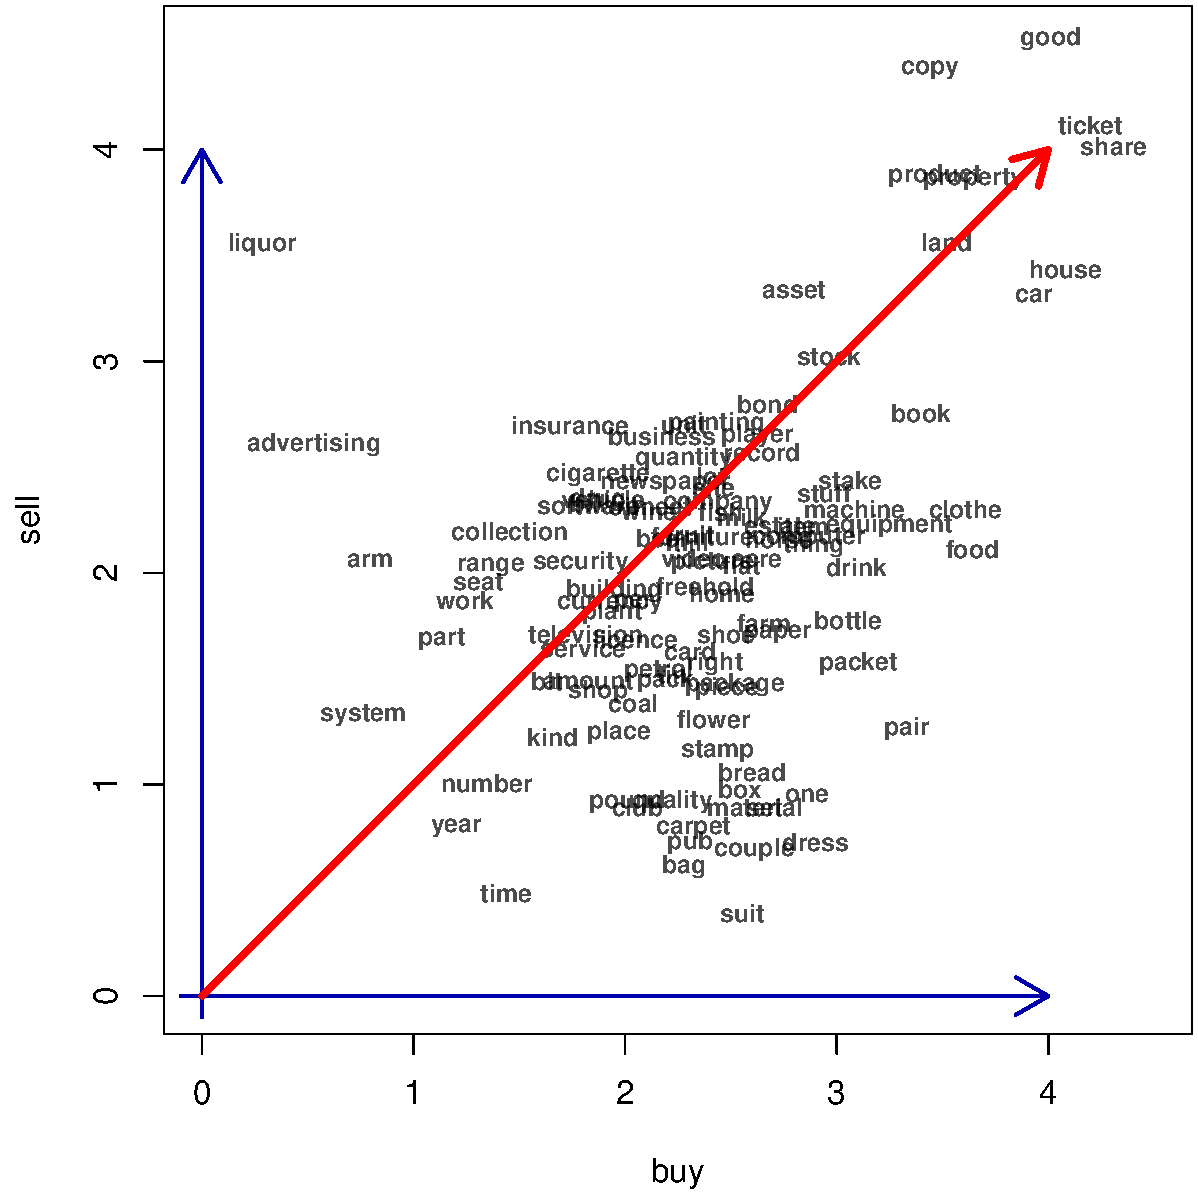
\includegraphics[width=8cm]{img/3_buy_sell_labels_latent}
  \end{center}
\end{frame}


%%%%%%%%%%%%%%%%%%%%%%%%%%%%%%%%%%%%%%%%%%
\subsection{Examples}

\begin{frame}
  \frametitle{Some well-known DSM examples}

  \ungap
  \begin{block} {Latent Semantic Analysis \citep{Landauer:Dumais:97}}
  \begin{itemize}
  \item term-context matrix with document context
  \item weighting: log term frequency and term entropy
  \item distance measure: cosine
  \item dimensionality reduction: SVD
  \end{itemize}
  \end{block}
 
 \begin{block} {Hyperspace Analogue to Language \citep{Lund:Burgess:96}}
  \begin{itemize}
  \item term-term matrix with surface context
  \item structured (left/right) and distance-weighted frequency counts
  \item distance measure: Minkowski metric ($1\leq p \leq 2$)
  \item dimensionality reduction: feature selection (high variance)
  \end{itemize}
  \end{block}
\end{frame}

\begin{frame}
  \frametitle{Some well-known DSM examples}

  \ungap
  \begin{block} {Infomap NLP \citep{Widdows:04}}
  \begin{itemize}
  \item term-term matrix with unstructured surface context
  \item weighting: none
  \item distance measure: cosine
  \item dimensionality reduction: SVD
  \end{itemize}
  \end{block}
 
  \begin{block} {Random Indexing \citep{Karlgren:Sahlgren:01}}
    \begin{itemize}
    \item term-term matrix with unstructured surface context
    \item weighting: various methods 
    \item distance measure: various methods
    \item dimensionality reduction: random indexing (RI)
    \end{itemize}
  \end{block}
\end{frame}

\begin{frame}
  \frametitle{Some well-known DSM examples}

  \ungap
  \begin{block}{Dependency Vectors \citep{Pado:Lapata:07}}
  \begin{itemize}
  \item term-term matrix with unstructured dependency context
  \item weighting: log-likelihood ratio
  \item distance measure: information-theoretic \citep{Lin:98a}
  \item dimensionality reduction: none
  \end{itemize}
  \end{block}
 
 \begin{block} {Distributional Memory \citep{Baroni:Lenci:10}}
  \begin{itemize}
  \item term-term matrix with structured and unstructered dependencies + knowledge patterns
  \item weighting: local-MI on type frequencies of link patterns
  \item distance measure: cosine
  \item dimensionality reduction: none
  \end{itemize}
  \end{block}
 \end{frame}

%%%%%%%%%%%%%%%%%%%%%%%%%%%%%%%%%%%%%%%%%%%%%%%%%%%%%%%%%%%%%%%%%%%%%%
\section{DSM in practice}

%%%%%%%%%%%%%%%%%%%%%%%%%%%%%%%%%%%%%%%%%%
\subsection{Using DSM distances}

\begin{frame}
  \frametitle{Nearest neighbours}
  \framesubtitle{DSM based on verb-object relations from BNC, reduced to 100 dim.\ with SVD}
  % \framesubtitle{}

  Neighbours of \h{dog} (cosine angle):
  \begin{itemize}\item[\hand]
    girl (45.5), boy (46.7), horse(47.0), wife (48.8), baby (51.9),
    daughter (53.1), side (54.9), mother (55.6), boat (55.7),
    rest (56.3), night (56.7), cat (56.8), son (57.0), man (58.2), 
    place (58.4), husband (58.5), thing (58.8), friend (59.6), \ldots
  \end{itemize}

  \gap
  Neighbours of \h{school}:
  \begin{itemize}\item[\hand]
    country (49.3), church (52.1), hospital (53.1), house (54.4),
    hotel (55.1), industry (57.0), company (57.0), home (57.7), family
    (58.4), university (59.0), party (59.4), group (59.5), building
    (59.8), market (60.3), bank (60.4), business (60.9), area (61.4),
    department (61.6), club (62.7), town (63.3), library (63.3), 
    room (63.6), service (64.4), police (64.7), \ldots
  \end{itemize}
  \addnote{Neighbours and neighbourhood plots from BNC verb-object DSM, reduced to 100 dimensions by SVD.}%
\end{frame}

\begin{frame}[c]
  \frametitle{Nearest neighbours}
  % \framesubtitle{}

  \ungap[1]
  \begin{center}
    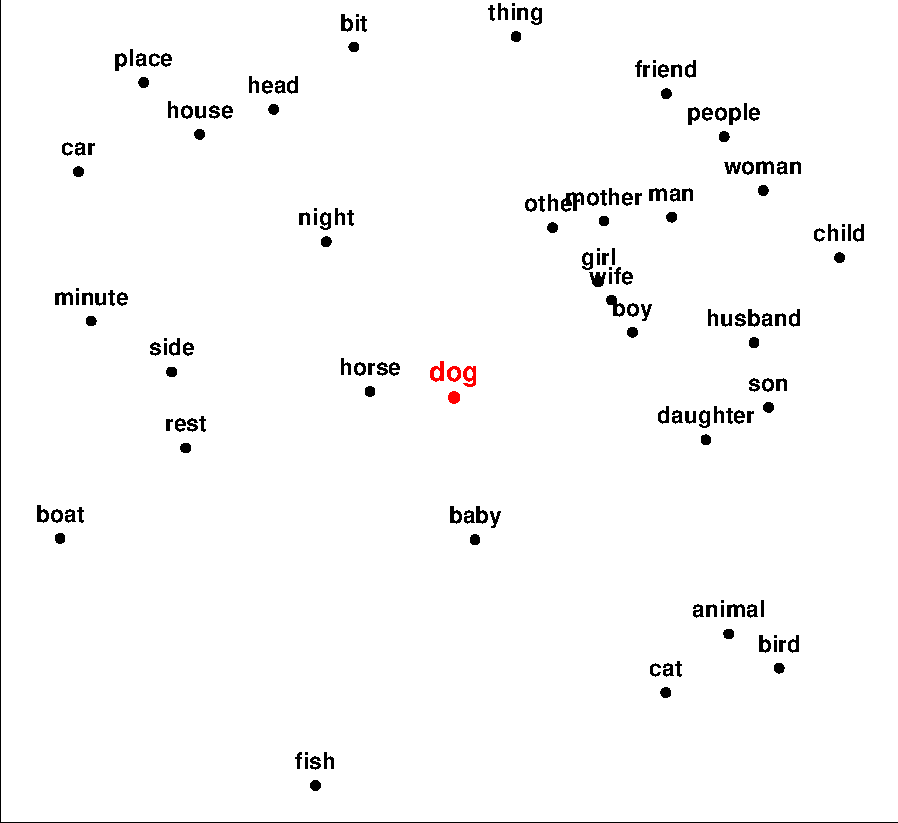
\includegraphics[width=8cm]{img/neighbourhood_dog}
  \end{center}
\end{frame}

\begin{frame}[c]
  \frametitle{Semantic maps}
  % \framesubtitle{}

  \begin{center}
    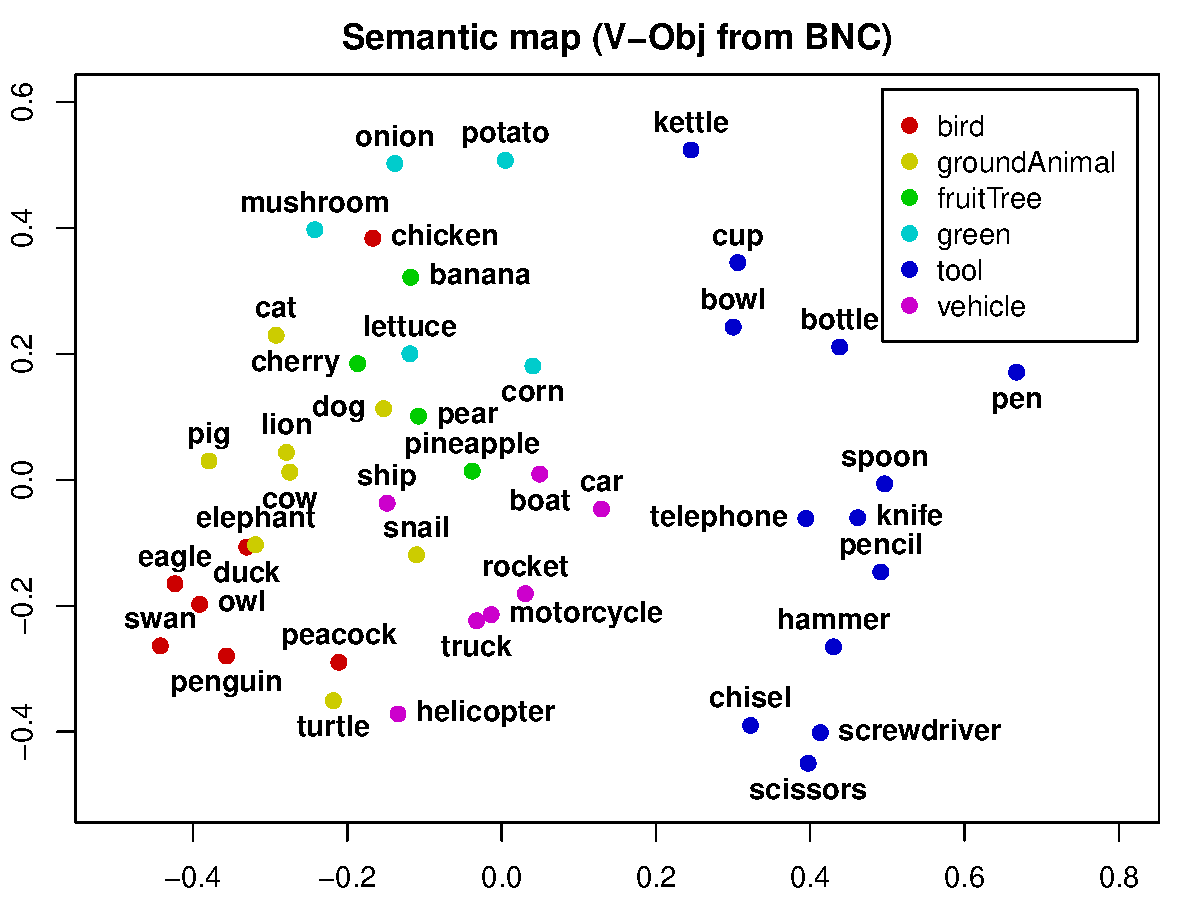
\includegraphics[width=100mm]{img/hieroglyph_semantic_map}
  \end{center}
\end{frame}

\begin{frame}[c]
  \frametitle{Clustering}
  % \framesubtitle{}

  \begin{center}
    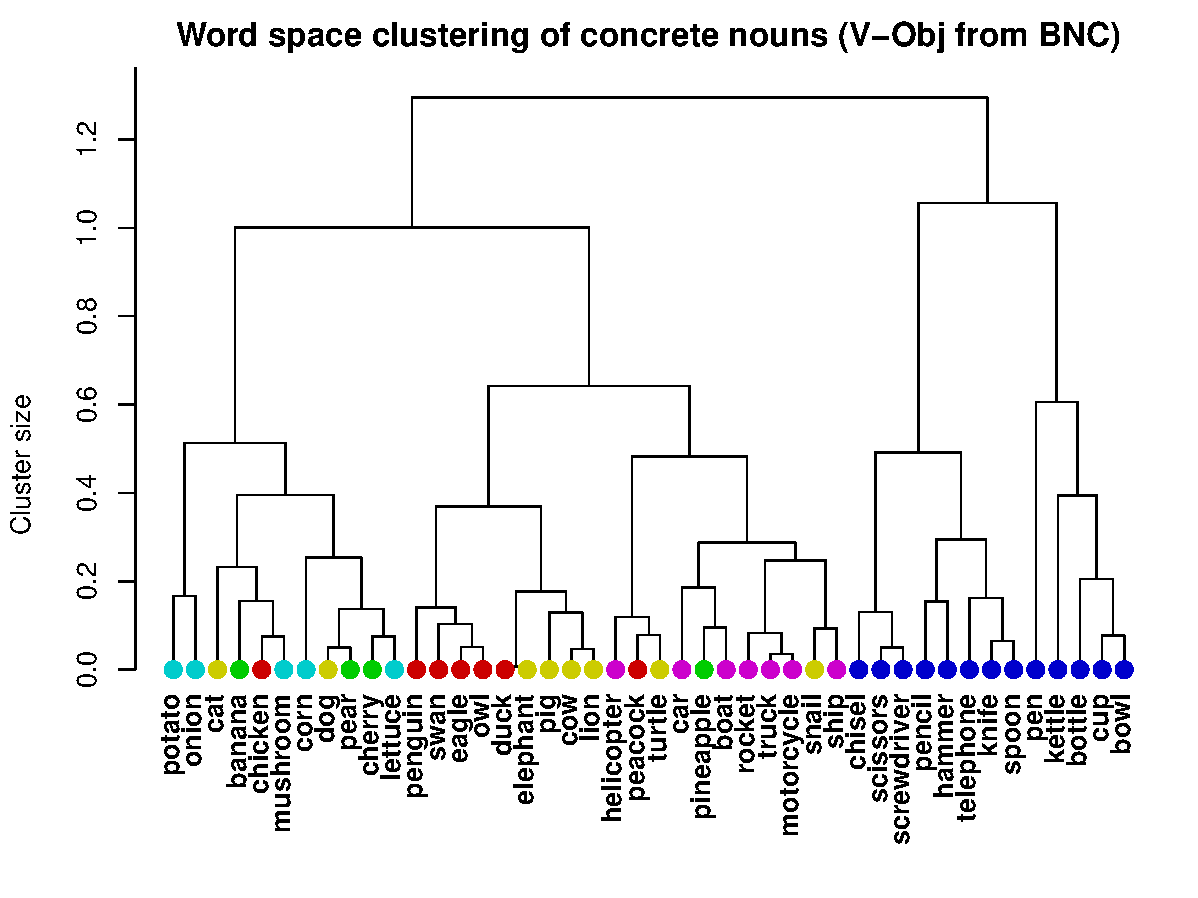
\includegraphics[width=100mm]{img/hieroglyph_clustering}
  \end{center}
\end{frame}

\begin{frame}[c]
  \frametitle{Latent dimensions}
  % \framesubtitle{}

  \begin{center}
    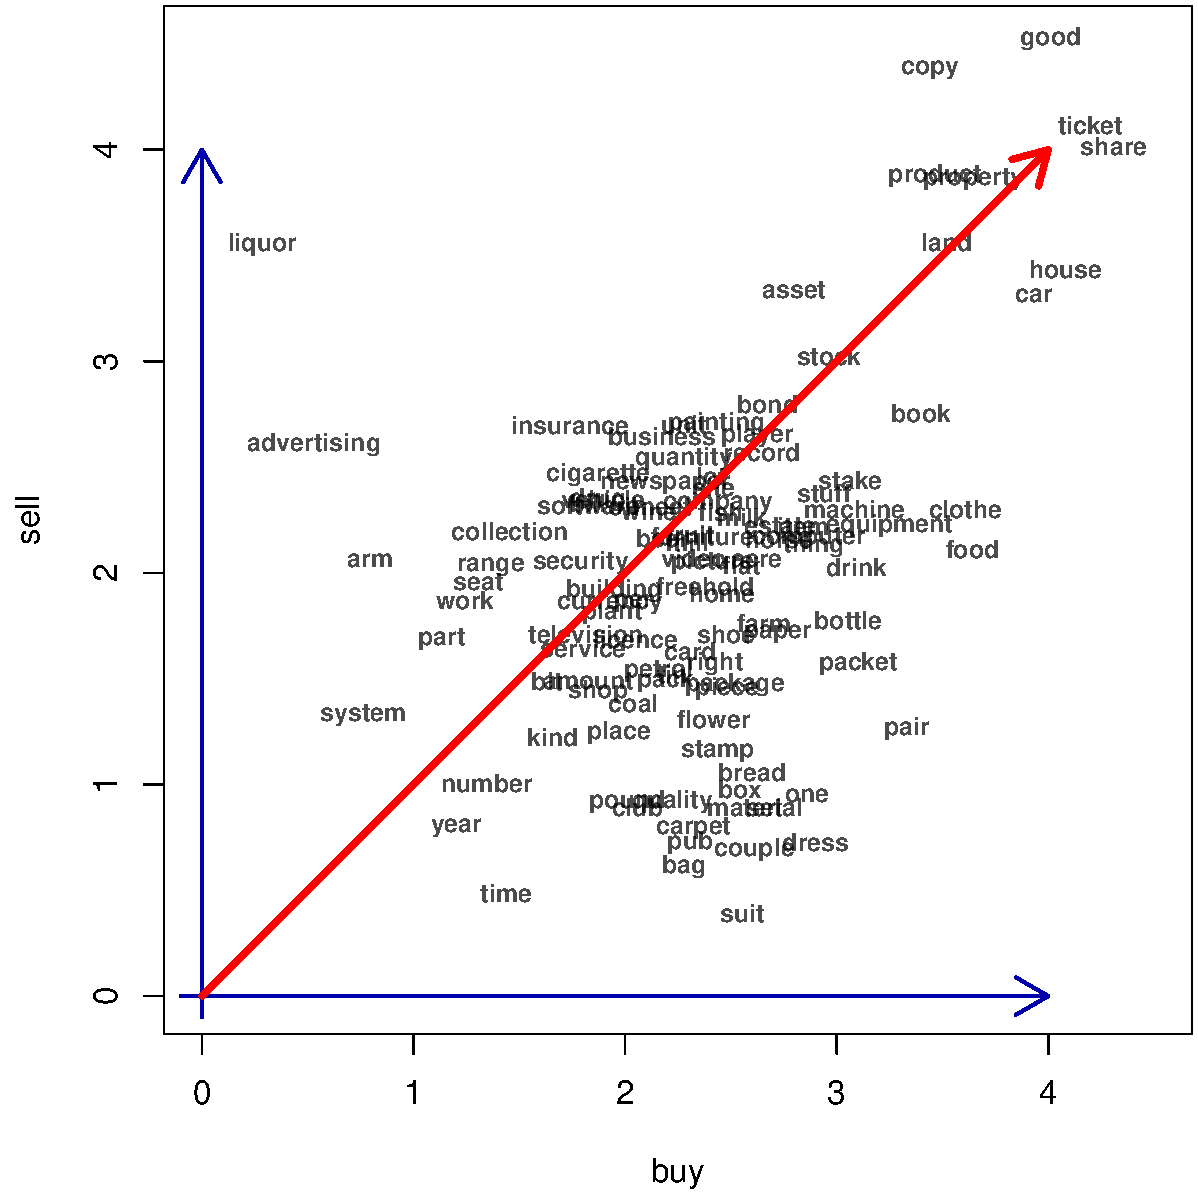
\includegraphics[width=8cm]{img/3_buy_sell_labels_latent}
  \end{center}
\end{frame}

\begin{frame}[c]
  \frametitle{Semantic similarity graph (topological structure)}
  % \framesubtitle{}

  \begin{center}
    \begin{tabular}{@{}cc@{}}
    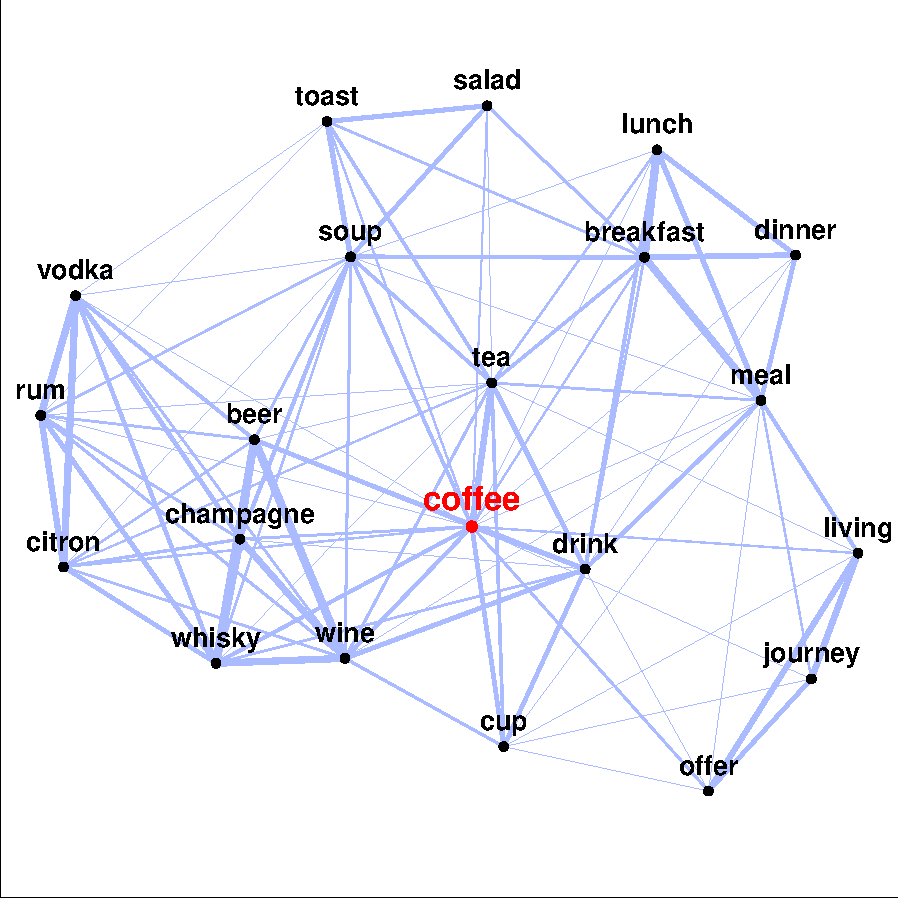
\includegraphics[width=55mm]{img/neighbourhood_coffee} &
    \visible<2->{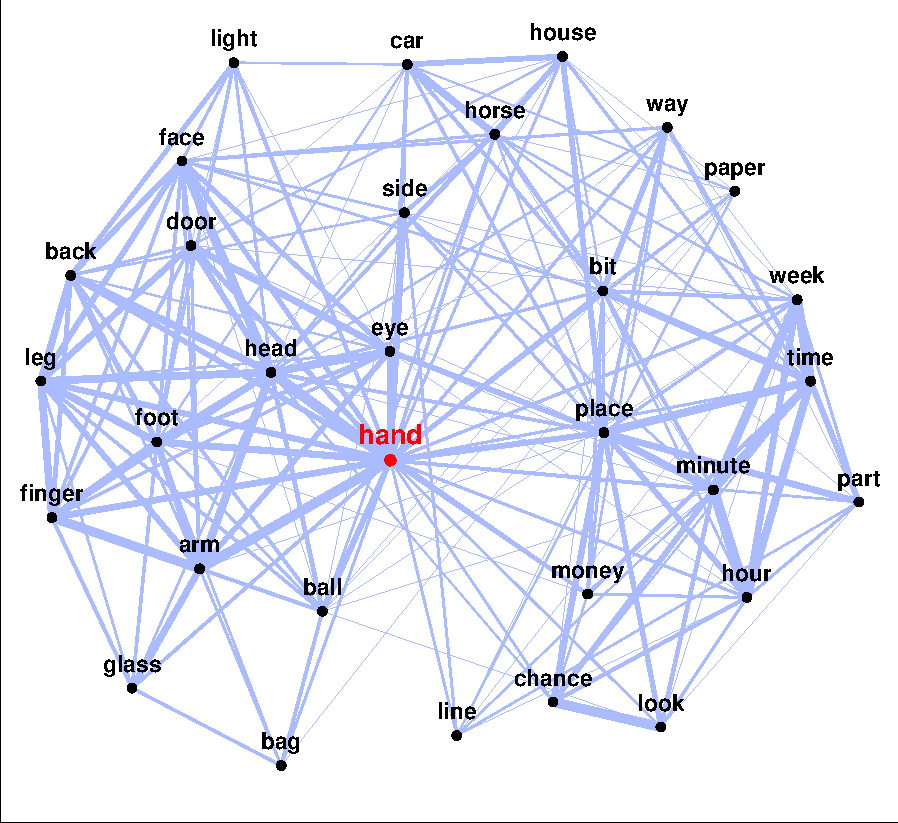
\includegraphics[width=55mm]{img/neighbourhood_hand}}
  \end{tabular}
  \end{center}
\end{frame}

\begin{frame}
  \frametitle{Context vectors \citep{Schuetze:98}}

  \gap
  \begin{columns}[c]
    \begin{column}{50mm}
      Distributional representation only at type level
      \begin{itemize}
      \item[\hand] What is the ``average'' meaning of \emph{mouse}? (computer \vs animal)
      \item[]
      \end{itemize}
      \pause
      \h{Context vector} approximates meaning of individual token
      \begin{itemize}
      \item \hh{bag-of-words} approach:
        centroid of all context words in the sentence
      \end{itemize}
    \end{column}
    \begin{column}{60mm}
      \includegraphics[width=60mm]{img/illustration_context_vectors_mouse}
    \end{column}
  \end{columns}
\end{frame}


%%%%%%%%%%%%%%%%%%%%%%%%%%%%%%%%%%%%%%%%%%
\subsection{Quantitative evaluation}

%%%%%%%%%%%%%%%%%%%%%%%%%%%%%%%%%%%%%%%%%%
%\subsection{Synonym identification and semantic similarity judgements}

\begin{frame}\frametitle{The TOEFL synonym task}

  \begin{itemize}
  \item The TOEFL dataset
    \begin{itemize}
    \item 80 items
    \item Target: \emph{levied}\\
      Candidates: \emph{believed, correlated, \alert<2->{imposed}, requested}
    \item<3-> Target \emph{fashion}\\
      Candidates: \emph{craze, fathom, \alert<4->{manner}, ration}
  \end{itemize}
    \item[]
  \item<5-> DSMs and TOEFL
  \begin{enumerate}
  \item take vectors of the target ($\Vector{t}$) and of the candidates
($\Vector{c}_1 \dots \Vector{c}_n$)
\item measure the distance between $\Vector{t}$ and $\Vector{c}_i$, with
$1 \leq i \leq n$ 
\item select $\Vector{c}_i$ with the shortest distance in space from $\Vector{t}$
\end{enumerate}
  \end{itemize}

\end{frame}


\begin{frame}
  \frametitle{Humans \vs machines on the TOEFL task}

  \begin{itemize}
  \item Average foreign test taker: 64.5\%
  \item<2-> Macquarie University staff (Rapp 2004):
    \begin{itemize}
    \item Average of 5 non-natives: 86.75\%
    \item Average of 5 natives: \primary{97.75\%}
    \item[]
    \end{itemize}
  \item<3-> Distributional semantics
    \begin{itemize}
    \item Classic LSA \citep{Landauer:Dumais:97}: 64.4\%
    \item Padó and Lapata's (\citeyear{Pado:Lapata:07}) dependency-based model: 73.0\%
    \item Distributional memory \citep{Baroni:Lenci:10}: 76.9\%
    \item Rapp's (\citeyear{Rapp:04a}) SVD-based model, lemmatized BNC: 92.5\%
    \item \citet{Bullinaria:Levy:12} carry out aggressive parameter optimization: \primary{100.0\%}
    \end{itemize}
  \end{itemize}

\end{frame}


\begin{frame}
\frametitle{Semantic similarity judgments}

\begin{itemize}
\item \citet{Rubenstein:Goodenough:65} collected similarity ratings for 65 noun pairs from 51 subjects on a 0--4 scale
  \begin{center}
    \begin{tabular}{llr}
      $w_1$ & $w_2$ & avg.\ rating\\
      \toprule
      \emph{car} & \emph{automobile} & \secondary{3.9}\\
      \emph{food} &  \emph{fruit}  & \secondary{2.7}\\
      \emph{cord} & \emph{smile} & \secondary{0.0}\\
    \end{tabular}
  \end{center}
  \gap
\item<2-> DSMs \vs\ Rubenstein \& Goodenough
  \begin{enumerate}
  \item for each test pair $(w_1, w_2)$, take vectors $\Vector{w}_1$ and $\Vector{w}_2$
  \item measure the distance (e.g.\ cosine) between $\Vector{w}_1$ and $\Vector{w}_2$
  \item measure (Pearson) correlation between vector distances and R\&G average judgments \citep{Pado:Lapata:07}
  \end{enumerate}
\end{itemize}
\end{frame}  

\begin{frame}
  \frametitle{Semantic similarity judgments: example}
  \ungap[1]
  \begin{center}
    \includegraphics[width=9cm]{img/bnc_rg65}
  \end{center}
\end{frame}

\begin{frame}
\frametitle{Semantic similarity judgments: results}

Results on RG65 task:
\begin{itemize}
\item Padó and Lapata's (\citeyear{Pado:Lapata:07}) dependency-based model: 0.62
\item Dependency-based on Web corpus \citep{Herdagdelen:Erk:Baroni:09}
  \begin{itemize}
  \item without SVD reduction: 0.69
  \item with SVD reduction: 0.80
  \end{itemize}
\item Distributional memory \citep{Baroni:Lenci:10}: 0.82
\item Salient Semantic Analysis \citep{Hassan:Mihalcea:11}: 0.86
\end{itemize}

\end{frame}

%%%%%%%%%%%%%%%%%%%%%%%%%%%%%%%%%%%%%%%%%%
\subsection{Software and further information}

\begin{frame}
  \frametitle{Software packages}

  \begin{tabular}{>{\color{secondary}}ll>{\itshape}p{6cm}}
    \href{http://www.psych.ualberta.ca/~westburylab/downloads/HiDEx.download.html}{HiDEx} & C++ & re-implementation of the HAL model \citep{Lund:Burgess:96} \\
    \href{http://code.google.com/p/semanticvectors/}{SemanticVectors} & Java & scalable architecture based on random indexing representation \\
    \href{http://github.com/fozziethebeat/S-Space}{S-Space} & Java & complex object-oriented framework \\
    \href{http://maggie.lt.informatik.tu-darmstadt.de/jobimtext/}{JoBimText} & Java & UIMA / Hadoop framework \\
    \href{http://radimrehurek.com/gensim/}{Gensim} & Python & complex framework, focus on parallelization and out-of-core algorithms \\
    \href{http://clic.cimec.unitn.it/composes/toolkit/}{DISSECT} & Python & user-friendly, designed for research on compositional semantics \\
    \href{http://wordspace.r-forge.r-project.org/}{\color{primary}\texttt{wordspace}} & R & interactive research laboratory, but scales to real-life data sets
  \end{tabular}

  \vspace{1em}
  \hfill\light{\small click on package name to open Web page}
\end{frame}

\begin{frame}
  \frametitle{Recent conferences and workshops}
  % \framesubtitle{}

  \ungap[1]
  \begin{itemize}
  \item \primary{2007}: \href{http://clic.cimec.unitn.it/marco/beyond_words/}{CoSMo Workshop} (at Context '07)
  \item \primary{2008}: \href{http://wordspace.collocations.de/doku.php/workshop:esslli:start}{ESSLLI Lexical Semantics Workshop} \& \href{http://wordspace.collocations.de/doku.php/workshop:esslli:task}{Shared Task}, \href{http://linguistica.sns.it/RdL/2008.html}{Special Issue of the Italian Journal of Linguistics}
  \item \primary{2009}: \href{http://art.uniroma2.it/gems/}{GeMS Workshop} (EACL 2009), \href{http://www.let.rug.nl/disco2009/}{DiSCo Workshop} (CogSci 2009), \href{http://wordspace.collocations.de/doku.php/course:esslli2009:start}{ESSLLI Advanced Course on DSM}
  \item \primary{2010}: \href{http://art.uniroma2.it/gems010/}{2nd GeMS} (ACL 2010), \href{http://clic.cimec.unitn.it/roberto/ESSLLI10-dsm-workshop/}{ESSLLI Workshop on Compositionality and DSM}, \href{http://naaclhlt2010.isi.edu/tutorials/t4.html}{DSM Tutorial} (NAACL 2010), \href{http://journals.cambridge.org/action/displayIssue?iid=7911772}{Special Issue of JNLE on Distributional Lexical Semantics}
  \item \primary{2011}: \href{http://disco2011.fzi.de}{2nd DiSCo} (ACL 2011), \href{https://sites.google.com/site/geometricalmodels/}{3rd GeMS} (EMNLP 2011)
  \item \primary{2012}: \href{http://didas.org}{DiDaS} (at ICSC 2012)
  \item \primary{2013}: \href{https://sites.google.com/site/cvscworkshop/}{CVSC} (ACL 2013), \href{http://clic.cimec.unitn.it/roberto/IWCS-TFDS2013/}{TFDS} (IWCS 2013), \href{http://www.dagstuhl.de/en/program/calendar/semhp/?semnr=13462}{Dagstuhl}
  \item \primary{2014}: \href{https://sites.google.com/site/cvscworkshop2014/}{2nd CVSC} (at EACL 2014)
  \end{itemize}
  \hfill\light{\small click on Workshop name to open Web page}
  \addnote{CoSMo = \underline{Co}ntextual Information in \underline{S}emantic Space \underline{M}odels}%
  \addnote{ESSLLI = European Summer School in Logic, Language and Information}%
  \addnote{GeMS = \underline{Ge}ometrical \underline{M}odels of Natural Language \underline{S}emantics}%
  \addnote{DiSCo = \underline{Di}stributional \underline{S}emantics beyond Concrete \underline{Co}ncepts}%
  \addnote{JNLE = Journal of Natural Language Engineering}%
  \addnote{DiSCo 2 = \underline{Di}stributional \underline{S}emantics and \underline{Co}mpositionality}%
  \addnote{DiDaS = Workshop on \underline{Di}stributional \underline{Da}ta \underline{S}emantics}%
  \addnote{CVSC = \underline{C}ontinuous \underline{V}ector \underline{S}pace Models and their \underline{C}ompositionality}%
  \addnote{TFDS = Towards a Formal Distributional Semantics}%
\end{frame}


\begin{frame}
  \frametitle{Further information}
  % \framesubtitle{}

  \begin{itemize}
  \item Handouts \& other materials available from wordspace wiki at
    \begin{center}
      \secondary{\url{http://wordspace.collocations.de/}}
    \end{center}
    \begin{itemize}
    \item[\hand] based on joint work with Marco Baroni and Alessandro Lenci
    \end{itemize}
  \item Tutorial is open source (CC), and can be downloaded from
    \begin{center}\small
      \secondary{\url{http://r-forge.r-project.org/projects/wordspace/}}
    \end{center}
    \gap[.5]
  \item Review paper on distributional semantics:
    \begin{itemize}
    \item[] \small\nocite{Turney:Pantel:10}
      Turney, Peter~D. and Pantel, Patrick (2010).
      \primary{From frequency to meaning: Vector space models of semantics.}
      {\em Journal of Artificial Intelligence Research}, {\bf 37}, 141--188.%
      \nocite{Turney:Pantel:10}
    \end{itemize}
    \gap[.5]
  \item I should be working on textbook \primary{\emph{Distributional Semantics}} for \secondary{\emph{Synthesis Lectures on HLT}} (Morgan \& Claypool)
  \end{itemize}

\end{frame}

%%%%%%%%%%%%%%%%%%%%%%%%%%%%%%%%%%%%%%%%%%%%%%%%%%%%%%%%%%%%%%%%%%%%%%
%% References (if any)

\frame[allowframebreaks]{
  \frametitle{References}
  \bibliographystyle{natbib-stefan}
  \begin{scriptsize}
    \bibliography{dsm}
  \end{scriptsize}
}

\end{document}
